\documentclass{beamer}

% chinese fonts
\usepackage{ctex}

% math fonts
\usepackage{amsmath}
\usepackage{amsthm}
\usepackage{amssymb}
\usepackage{bm}

% figures
\usepackage{tikz}
\usepackage{graphicx}
\graphicspath{{./figures/}}

% tables
\usepackage{tabularx}
\usepackage{booktabs}
\usepackage{multirow}

\usepackage{enumerate}

% hyperlinks
\usepackage{hyperref}
% \hypersetup{
%   breaklinks,
%   colorlinks = true,
%   citecolor  = blue,
%   linkcolor  = white,
%   urlcolor   = magenta,
% }

% algorithms
% \makeatletter
%   \newif\if@restonecol
% \makeatother
% \let\algorithm\relax
% \let\endalgorithm\relax
\usepackage[linesnumbered,ruled,lined]{algorithm2e}
\usepackage{algpseudocode}
\renewcommand{\algorithmicrequire}{\textbf{Input:}}  % Use Input in the format of Algorithm
\renewcommand{\algorithmicensure}{\textbf{Output:}} % Use Output in the format of Algorithm

% bibliography
\usepackage[sort&compress,numbers]{natbib}

\usepackage[T1]{fontenc}

% other packages
\usepackage{latexsym,xcolor,multicol,calligra}
\usepackage{pstricks,listings,stackengine}

% About:  Macros for Vector, Matrix, Tensor, Math Operator and Misc
% Author: Jingxuan Yang

% vectors
\newcommand{\va}{\bm{a}}       \newcommand{\vah}{\hat{\bm{a}}}        \newcommand{\ah}{\hat{a}}    \newcommand{\vat}{\tilde{\bm{a}}}       \newcommand{\at}{\tilde{a}}
\newcommand{\vb}{\bm{b}}       \newcommand{\vbh}{\hat{\bm{b}}}        \newcommand{\bh}{\hat{b}}    \newcommand{\vbt}{\tilde{\bm{b}}}       \newcommand{\bt}{\tilde{b}}
\newcommand{\vc}{\bm{c}}       \newcommand{\vch}{\hat{\bm{c}}}        \newcommand{\ch}{\hat{c}}    \newcommand{\vct}{\tilde{\bm{c}}}       \newcommand{\ct}{\tilde{c}}
\newcommand{\vd}{\bm{d}}       \newcommand{\vdh}{\hat{\bm{d}}}        \newcommand{\dhat}{\hat{d}}  \newcommand{\vdt}{\tilde{\bm{d}}}       \newcommand{\dt}{\tilde{d}}
\newcommand{\ve}{\bm{e}}       \newcommand{\veh}{\hat{\bm{e}}}        \newcommand{\eh}{\hat{e}}    \newcommand{\vet}{\tilde{\bm{e}}}       \newcommand{\et}{\tilde{e}}
\newcommand{\vf}{\bm{f}}       \newcommand{\vfh}{\hat{\bm{f}}}        \newcommand{\fh}{\hat{f}}    \newcommand{\vft}{\tilde{\bm{f}}}       \newcommand{\ft}{\tilde{f}}
\newcommand{\vg}{\bm{g}}       \newcommand{\vgh}{\hat{\bm{g}}}        \newcommand{\gh}{\hat{g}}    \newcommand{\vgt}{\tilde{\bm{g}}}       \newcommand{\gt}{\tilde{g}}
\newcommand{\vech}{\bm{h}}     \newcommand{\vhh}{\hat{\bm{h}}}        \newcommand{\hh}{\hat{h}}    \newcommand{\vht}{\tilde{\bm{h}}}       \newcommand{\htild}{\tilde{h}}
\newcommand{\vi}{\bm{i}}       \newcommand{\vih}{\hat{\bm{i}}}        \newcommand{\ih}{\hat{i}}    \newcommand{\vit}{\tilde{\bm{i}}}       \newcommand{\itild}{\tilde{i}}
\newcommand{\vj}{\bm{j}}       \newcommand{\vjh}{\hat{\bm{j}}}        \newcommand{\jh}{\hat{j}}    \newcommand{\vjt}{\tilde{\bm{j}}}       \newcommand{\jt}{\tilde{j}}
\newcommand{\vk}{\bm{k}}       \newcommand{\vkh}{\hat{\bm{k}}}        \newcommand{\kh}{\hat{k}}    \newcommand{\vkt}{\tilde{\bm{k}}}       \newcommand{\kt}{\tilde{k}}
\newcommand{\vl}{\bm{l}}       \newcommand{\vlh}{\hat{\bm{l}}}        \newcommand{\lh}{\hat{l}}    \newcommand{\vlt}{\tilde{\bm{l}}}       \newcommand{\lt}{\tilde{l}}
\newcommand{\vm}{\bm{m}}       \newcommand{\vmh}{\hat{\bm{m}}}        \newcommand{\mh}{\hat{m}}    \newcommand{\vmt}{\tilde{\bm{m}}}       \newcommand{\mt}{\tilde{m}}
\newcommand{\vn}{\bm{n}}       \newcommand{\vnh}{\hat{\bm{n}}}        \newcommand{\nh}{\hat{n}}    \newcommand{\vnt}{\tilde{\bm{n}}}       \newcommand{\nt}{\tilde{n}}
\newcommand{\vo}{\bm{o}}       \newcommand{\voh}{\hat{\bm{o}}}        \newcommand{\oh}{\hat{o}}    \newcommand{\vot}{\tilde{\bm{o}}}       \newcommand{\ot}{\tilde{o}}
\newcommand{\vp}{\bm{p}}       \newcommand{\vph}{\hat{\bm{p}}}        \newcommand{\ph}{\hat{p}}    \newcommand{\vpt}{\tilde{\bm{p}}}       \newcommand{\pt}{\tilde{p}}
\newcommand{\vq}{\bm{q}}       \newcommand{\vqh}{\hat{\bm{q}}}        \newcommand{\qh}{\hat{q}}    \newcommand{\vqt}{\tilde{\bm{q}}}       \newcommand{\qt}{\tilde{q}}
\newcommand{\vr}{\bm{r}}       \newcommand{\vrh}{\hat{\bm{r}}}        \newcommand{\rh}{\hat{r}}    \newcommand{\vrt}{\tilde{\bm{r}}}       \newcommand{\rt}{\tilde{r}}
\newcommand{\vs}{\bm{s}}       \newcommand{\vsh}{\hat{\bm{s}}}        \newcommand{\sh}{\hat{s}}    \newcommand{\vst}{\tilde{\bm{s}}}       \newcommand{\st}{\tilde{s}}
\newcommand{\vt}{\bm{t}}       \newcommand{\vth}{\hat{\bm{t}}}        \newcommand{\that}{\hat{t}}  \newcommand{\vtt}{\tilde{\bm{t}}}       \newcommand{\ttil}{\tilde{t}}
\newcommand{\vu}{\bm{u}}       \newcommand{\vuh}{\hat{\bm{u}}}        \newcommand{\uh}{\hat{u}}    \newcommand{\vut}{\tilde{\bm{u}}}       \newcommand{\ut}{\tilde{u}}
\newcommand{\vv}{\bm{v}}       \newcommand{\vvh}{\hat{\bm{v}}}        \newcommand{\vh}{\hat{v}}    \newcommand{\vvt}{\tilde{\bm{v}}}       \newcommand{\vtild}{\tilde{v}}
\newcommand{\vw}{\bm{w}}       \newcommand{\vwh}{\hat{\bm{w}}}        \newcommand{\wh}{\hat{w}}    \newcommand{\vwt}{\tilde{\bm{w}}}       \newcommand{\wt}{\tilde{w}}
\newcommand{\vx}{\bm{x}}       \newcommand{\vxh}{\hat{\bm{x}}}        \newcommand{\xh}{\hat{x}}    \newcommand{\vxt}{\tilde{\bm{x}}}       \newcommand{\xt}{\tilde{x}}
\newcommand{\vy}{\bm{y}}       \newcommand{\vyh}{\hat{\bm{y}}}        \newcommand{\yh}{\hat{y}}    \newcommand{\vyt}{\tilde{\bm{y}}}       \newcommand{\yt}{\tilde{y}}
\newcommand{\vz}{\bm{z}}       \newcommand{\vzh}{\hat{\bm{z}}}        \newcommand{\zh}{\hat{z}}    \newcommand{\vzt}{\tilde{\bm{z}}}       \newcommand{\zt}{\tilde{z}}

\newcommand{\valpha}{\bm{\alpha}}
\newcommand{\vbeta}{\bm{\beta}}
\newcommand{\vgamma}{\bm{\gamma}}
\newcommand{\vtheta}{\bm{\theta}}
\newcommand{\vlambda}{\bm{\lambda}}
\newcommand{\vmu}{\bm{\mu}}
\newcommand{\vomega}{\bm{\omega}}
\newcommand{\vxi}{\bm{\xi}}
\newcommand{\veta}{\bm{\eta}}
\newcommand{\vvarepsilon}{\bm{\varepsilon}}

\newcommand{\mSigma}{\bm{\Sigma}}
\newcommand{\mLambda}{\bm{\Lambda}}

\newcommand{\Ac}{\mathcal{A}}
\newcommand{\Fc}{\mathcal{F}}
\newcommand{\Xc}{\mathcal{X}}
\newcommand{\Yc}{\mathcal{Y}}
\newcommand{\Zc}{\mathcal{Z}}
\newcommand{\Gc}{\mathcal{G}}
\newcommand{\Hc}{\mathcal{H}}
\newcommand{\Dc}{\mathcal{D}}
\newcommand{\Cc}{\mathcal{C}}
\newcommand{\Rc}{\mathcal{R}}
\newcommand{\Nc}{\mathcal{N}}

% matrices
\newcommand{\ma}{\bm{A}}
\newcommand{\mb}{\bm{B}}
\newcommand{\mc}{\bm{C}}
\newcommand{\md}{\bm{D}}
\newcommand{\mE}{\bm{E}}
\newcommand{\mf}{\bm{F}}
\newcommand{\mg}{\bm{G}}
\newcommand{\mH}{\bm{H}}
\newcommand{\mi}{\bm{I}}
\newcommand{\mj}{\bm{J}}
\newcommand{\mk}{\bm{K}}
\newcommand{\ml}{\bm{L}}
\newcommand{\mM}{\bm{M}}
\newcommand{\mn}{\bm{N}}
\newcommand{\mO}{\bm{O}}
\newcommand{\mP}{\bm{P}}
\newcommand{\mq}{\bm{Q}}
\newcommand{\mr}{\bm{R}}
\newcommand{\ms}{\bm{S}}
\newcommand{\mT}{\bm{T}}
\newcommand{\mU}{\bm{U}}
\newcommand{\mv}{\bm{V}}
\newcommand{\mw}{\bm{W}}
\newcommand{\mx}{\bm{X}}
\newcommand{\my}{\bm{Y}}
\newcommand{\mz}{\bm{Z}}

% tensors
\newcommand{\tp}{\mathsf{P}}
\newcommand{\tu}{\mathsf{U}}
\newcommand{\tx}{\mathsf{X}}
\newcommand{\ty}{\mathsf{Y}}
\newcommand{\tz}{\mathsf{Z}}
\newcommand{\tw}{\mathsf{W}}

% norms
\newcommand{\mynorm}[2]{\| {#1} \|_{#2}}
\newcommand{\norm}[2]{\mynorm{#1}{#2}}
\newcommand{\bignorm}[2]{\left\| {#1} \right\|_{#2}}
\newcommand{\norml}[1]{\mynorm{#1}{1}}
\newcommand{\bignorml}[1]{\bignorm{#1}{1}}
\newcommand{\infnorm}[1]{\mynorm{#1}{\infty}}
\newcommand{\biginfnorm}[1]{\bignorm{#1}{\infty}}
\newcommand{\oneinf}{\ell_{1,\infty}}
\newcommand{\onetwo}{\ell_{1,2}}
\newcommand{\oneinfnorm}[1]{\mynorm{#1}{1,\infty}}
\newcommand{\bigoneinf}[1]{\bignorm{#1}{1,\infty}}
\newcommand{\onetwonorm}[1]{\mynorm{#1}{1,2}}
\newcommand{\bigonetwo}[1]{\bignorm{#1}{1,2}}
\newcommand{\enorm}[1]{\mynorm{#1}{2}}
\newcommand{\bigenorm}[1]{\bignorm{#1}{2}}
\newcommand{\znorm}[1]{\mynorm{#1}{0}}
\newcommand{\bigznorm}[1]{\bignorm{#1}{0}}
\newcommand{\frob}[1]{\|{#1}\|_{\text{F}}}
\newcommand{\bigfrob}[1]{\bignorm{#1}{\text{F}}}
\newcommand{\grpnorm}[2]{\norm{#1}{\text{Gr}(#2)}}

% math operators
\DeclareMathOperator*{\argmin}{argmin}
\DeclareMathOperator*{\argmax}{argmax}
\DeclareMathOperator{\divg}{div}
\DeclareMathOperator{\dom}{dom}
\DeclareMathOperator{\interior}{int}
\DeclareMathOperator{\ri}{ri}
\DeclareMathOperator{\sgn}{sgn}
\DeclareMathOperator{\trace}{tr}
\DeclareMathOperator{\diag}{diag}
\DeclareMathOperator{\rank}{rank}
\DeclareMathOperator{\range}{Range}
\DeclareMathOperator{\vect}{vec}
\DeclareMathOperator{\prox}{prox}
\DeclareMathOperator{\intr}{int}
\DeclareMathOperator{\relint}{ri}
\DeclareMathOperator{\image}{Im}
\DeclareMathOperator{\kernal}{Ker}
\let\span\relax
\DeclareMathOperator{\span}{Span}
\DeclareMathOperator{\var}{Var}
\DeclareMathOperator{\cov}{Cov}

% misc
\newcommand{\gs}{\geqslant}
\newcommand{\ls}{\leqslant}
\newcommand{\set}[1]{\left\{ {#1}\right\}}

\newcommand{\defeq}{\ \stackrel{\text{def}}{=}\ }
\newcommand{\ip}[2]{\left\langle#1, #2\right\rangle}
\newcommand{\reals}{\mathbb{R}}
\newcommand{\complex}{\mathbb{C}}
\newcommand{\E}{\mathbb{E}}
\newcommand{\hop}{\mathrm{H}}
\renewcommand{\i}{\mathrm{i}}
\renewcommand{\j}{\mathrm{j}}
\newcommand{\half}{\frac{1}{2}}

\newtheorem{theorem}{Theorem}
\newtheorem{lemma}[theorem]{Lemma}
\newtheorem{proposition}[theorem]{Proposition}
\newtheorem{remark}[theorem]{Remark}
\newtheorem{corollary}[theorem]{Corollary}
\newtheorem{definition}[theorem]{Definition}


\usepackage{Tsinghua}

% defs
\def\cmd#1{\texttt{\color{red}\footnotesize $\backslash$#1}}
\def\env#1{\texttt{\color{blue}\footnotesize #1}}
\definecolor{deepblue}{rgb}{0,0,0.5}
\definecolor{deepred}{rgb}{0.6,0,0}
\definecolor{deepgreen}{rgb}{0,0.5,0}
\definecolor{halfgray}{gray}{0.55}

\lstset{
  basicstyle=\ttfamily\small,
  keywordstyle=\bfseries\color{deepblue},
  emphstyle=\ttfamily\color{deepred},    % Custom highlighting style
  stringstyle=\color{deepgreen},
  numbers=left,
  numberstyle=\small\color{halfgray},
  rulesepcolor=\color{red!20!green!20!blue!20},
  frame=shadowbox,
}

\author{杨敬轩, 董泽委}
\title{Low-Rank Matrix Restoration}
\subtitle{《矩阵分析》综合课题研究}
\institute[智能交通实验室]{系统工程研究所, 智能交通实验室}
\date{\today}

\begin{document}

\heiti
\begin{frame}
  \titlepage
  \begin{figure}[htpb]
    \centering
    
\includegraphics[width=0.19\linewidth]{THU_logo.pdf}
  \end{figure}
\end{frame}

\begin{frame}{目录}
  \begin{columns}[t]
    \begin{column}{.45\textwidth}
      \tableofcontents[sections={1-4},hideallsubsections]
    \end{column}
    \begin{column}{.45\textwidth}
      \tableofcontents[sections={5-8},hideallsubsections]
    \end{column}
  \end{columns}
\end{frame}

% \begin{frame}{目录}
%   \begin{multicols}{2}
%     \tableofcontents[hideallsubsections]
%   \end{multicols}
% \end{frame}

% \begin{frame}
%     \tableofcontents[sectionstyle=show,subsectionstyle=show/shaded/hide,subsubsectionstyle=show/shaded/hide]
% \end{frame}


\section{引言}

\begin{frame}{引言}
  \begin{block}{低秩矩阵恢复}
    \begin{itemize}
      \item 在计算机视觉与模式识别任务中, 通常都假设观测数据近似存在于一个低维的子空间下.
      \item 为找出这样的子空间, 经典的主成分分析 (Principal Component Analysis, PCA) \cite{abdi2010principal} 方法假定数据受到较小的高斯噪声污染, 即数据 $\mM\in\reals^{m\times n}$ 由一个低秩矩阵 $\ml\in\reals^{m\times n}$ 和一个独立同分布的高斯噪声矩阵 $\ms\in\reals^{m\times n}$ 构成.
      \item 当给定超参数 $r\in\mathbb{N}_{>0}$ 时, 该任务可以建模为优化问题: 
      \begin{equation}
        \begin{aligned}
          &\min_{\ml,\ms}~\|\ms\|_{\text{F}} \\
          &~\text{s.t.}~\rank(\ml)\leqslant r,\\
          &\qquad \mM=\ml+\ms.
        \end{aligned}
      \end{equation}
    \end{itemize}
  \end{block}
\end{frame}

\begin{frame}{引言}
  \begin{block}{低秩矩阵恢复}
    \begin{itemize}
      \item 在实际应用中, 若出现较高幅度的尖锐噪声或严重的离群点时, PCA 的性能会受到很大的影响.
      \item 当噪声矩阵 $\ms$ 足够稀疏时, 原始低秩矩阵仍然可能被恢复.
      \item 该任务可以建模为如下优化问题: 
      \begin{equation}
        \begin{aligned}
          &\min_{\ml,\ms}~\rank(\ml)+\lambda\|\ms\|_0 \\
          &~\text{s.t.}~~\mM=\ml+\ms,
        \end{aligned}
      \end{equation}
      其中, $\|\ms\|_0$ 指矩阵中非零元素的个数.
      \item 由于 $\rank(\ml)$ 和 $\|\ms\|_0$ 都是非凸的, 直接优化该问题非常困难, 因此需要对其进行凸松弛. 
    \end{itemize}
  \end{block}
\end{frame}

\begin{frame}{引言}
  \begin{block}{低秩矩阵恢复}
    鲁棒主成分分析 (Robust Principal Component Analysis, RPCA) \cite{candes2011robust} 提出将 $\rank(\ml)$ 用核范数 $\|\ml\|_{*}=\trace(\sqrt{\ml^\top\ml})$ 进行松弛, 并将 $\|\ms\|_0$ 用矩阵 $m_1$ 范数 $\|\ms\|_{m_1}=\sum_{i,j}|s_{i,j}|$ 进行松弛, 从而有
    \begin{equation}
      \label{eq:rpca}
      \begin{aligned}
        &\min_{\ml,\ms}~\|\ml\|_{*}+\lambda\|\ms\|_{m_1} \\
        &~\text{s.t.}~~\mM=\ml+\ms.
      \end{aligned}
    \end{equation}
  \end{block}
\end{frame}

\begin{frame}{引言}
  \begin{block}{主要贡献}
    \begin{itemize}
      \item 鲁棒主成分分析: 通用算法
      \begin{itemize}
        \item Gradient descent
        \item Gradient descent with Adam
      \end{itemize}
      \item 鲁棒主成分分析: 特殊算法
      \begin{itemize}
        \item Singular value thresholding
        \item Accelerated proximal gradient
        \item Augmented Lagrange multipliers
      \end{itemize}
      \item 矩阵补全
      \begin{itemize}
        \item Singular value thresholding
        \item Alternating direction method
        \item Alternating least squares
        \item Neural tangent kernels
      \end{itemize}
    \end{itemize}
  \end{block}
\end{frame}

\begin{frame}{引言}
  \begin{block}{GitHub Repository}
    \begin{itemize}
      \item Low-Rank Matrix Restoration
      
      {\color{purple}\footnotesize\url{https://github.com/jingxuanyang/LowRankMatrixRestoration}}

      \item 报告: \texttt{doc/report.pdf}
      \item 展示: \texttt{pre/slide.pdf}
      \item 说明: \texttt{README.md}
    \end{itemize}
  \end{block}
\end{frame}

\section[RPCA: 通用算法]{鲁棒主成分分析: 通用算法}

\subsection{Gradient descent}

\begin{frame}{鲁棒主成分分析: 通用算法}
  \begin{block}{Gradient descent}
    \begin{itemize}
      \item 梯度下降算法是一种求解优化问题的通用方法.
      \item 由式 (\ref{eq:rpca}) 给出的 RPCA 问题的优化目标中包含核范数和 $m_1$ 范数两项, 而这两项均不可导, 则需使用其次梯度 (Subgradient) \cite{boyd2003subgradient} 进行梯度下降.
      \item 对式 (\ref{eq:rpca}) 进行变形可得
      \begin{equation}
        \min_{\ml}~f(\ml)=\|\ml\|_{*}+\lambda\|\mM-\ml\|_{m_1}.
      \end{equation}
    \end{itemize}
  \end{block}
\end{frame}

\begin{frame}{鲁棒主成分分析: 通用算法}
  \begin{block}{Gradient descent}
    \begin{itemize}
      \item 令 $\ml=\mU\mSigma\mv^\top$ 为矩阵 $\ml$ 的 SVD 分解, 则核范数的次梯度 \cite{watson1992characterization,diadochos2018derivative} 为
      \begin{equation}
        \partial\|\ml\|_{*}=\{\mU\mv^\top+\mw:\mU^\top\mw=\mO,\mw\mv=\mO,\|\mw\|_2\leqslant1\}.
      \end{equation}
      \item 矩阵 $m_1$ 范数的次梯度可取为
      \begin{equation}
        -\sgn(\mM-\ml)\in\partial\|\mM-\ml\|_{m_1}.
      \end{equation}
      \item 目标函数 $f(\ml)$ 的次梯度可取为
      \begin{equation}
        \label{eq:subgradient}
        \mg=\mU\mv^\top-\sgn(\mM-\ml).
      \end{equation}
    \end{itemize}
  \end{block}
\end{frame}

\begin{frame}{鲁棒主成分分析: 通用算法}
  梯度下降算法如 Algorithm \ref{alg:gradient_descent} 所示.
  \begin{algorithm}[H]
    \small
    \label{alg:gradient_descent}
    \caption{Gradient descent for RPCA.}
    \KwIn{Data matrix $\mM$, learning rate $\alpha$, max iterations $T$, tolerance $\tau$}
    \KwOut{Low-rank matrix $\ml$, sparse noise matrix $\ms$}
    initialize $t=0$, $\ml=\mO$, terminate = False\;
    \While{not terminate and $t<T$}{
      $t \leftarrow t+1$\;
      $\mg \leftarrow \text{Subgradient}(\ml)$ by Eq.~(\ref{eq:subgradient})\;
      $\ml' \leftarrow \ml-\alpha\mg$\;
      $\text{terminate} \leftarrow |f(\ml') - f(\ml)| < \tau$\;
      $\ml \leftarrow \ml'$\;
    }
    $\ms \leftarrow \mM-\ml$\;
    return $\ml$, $\ms$\;
  \end{algorithm}
\end{frame}

\subsection{Gradient descent with Adam}

\begin{frame}{鲁棒主成分分析: 通用算法}
  采用 Adam \cite{kingma2014adam} 算法进行优化, 如 Algorithm \ref{alg:gradient_descent_adam} 所示.
  \begin{algorithm}[H]
    \small
    \label{alg:gradient_descent_adam}
    \caption{Gradient descent with Adam for RPCA.}
    \KwIn{Data matrix $\mM$, learning rate $\alpha$, max iterations $T$, tolerance $\tau$}
    \KwOut{Low-rank matrix $\ml$, sparse noise matrix $\ms$}
    set $\beta_1=0.9$, $\beta_2=0.999$, $\epsilon=10^{-8}$\;
    initialize $t=0$, $\ml=\mO$, terminate = False, $\mw_0=\mv_0=\mO$\;
    \While{not terminate and $t<T$}{
      $t \leftarrow t+1$,
      $\mg \leftarrow \text{Subgradient}(\ml)$ by Eq.~(\ref{eq:subgradient})\;
      $\mw_t\leftarrow\beta_1\mw_{t-1}+(1-\beta_1)\mg$,
      $\mv_t\leftarrow\beta_2\mv_{t-1}+(1-\beta_2)\mg\odot\mg$\;
      $\hat{\mw}_t\leftarrow \mw_t/(1-\beta_1^t)$,
      $\hat{\mv}_t\leftarrow \mv_t/(1-\beta_2^t)$\;
      $\ml' \leftarrow \ml-\alpha\hat{\mw}_t\oslash(\sqrt{\hat{\mv}_t}+\epsilon)$ \qquad /* $\sqrt{\cdot}$ applied element-wise */\;
      $\text{terminate} \leftarrow |f(\ml') - f(\ml)| < \tau$,
      $\ml \leftarrow \ml'$\;
    }
    $\ms \leftarrow \mM-\ml$\;
    return $\ml$, $\ms$\;
  \end{algorithm}
\end{frame}

\section[RPCA: 特殊算法]{鲁棒主成分分析: 特殊算法}
\label{sec:rpca_special}

\subsection{Preliminaries}

\begin{frame}{鲁棒主成分分析: 特殊算法}
  \begin{block}{Preliminaries}
    \begin{itemize}
      \item 设 $\mq\in\reals^{m\times n}$, 则优化问题
      \begin{equation}
        \min_{\mx}~\epsilon\|\mx\|_{m_1}+\frac{1}{2}\|\mx-\mq\|_{\text{F}}^2
      \end{equation}
      的最优解为 $\mx^*=\mathcal{S}_\epsilon(\mq)$ \cite{candes2011robust}.
      \item 其中 $\mathcal{S}_\epsilon$ 为 Shrinkage 算子,
      \begin{equation}
        \mathcal{S}_\epsilon(\mq)=\max(|\mq|-\epsilon, 0)\odot\sgn(\mq).
      \end{equation}
      \item 上述 $\max()$, $\sgn()$ 运算均为按元素进行 (element-wise) 的运算.
    \end{itemize}
  \end{block}
\end{frame}

\begin{frame}{鲁棒主成分分析: 特殊算法}
  \begin{block}{Preliminaries}
    \begin{itemize}
      \item 将 $m_1$ 范数替换为核范数, 则有
      \begin{equation}
        \min_{\mx}~\epsilon\|\mx\|_{*}+\frac{1}{2}\|\mx-\mq\|_{\text{F}}^2.
      \end{equation}
      \item 其闭式解为 $\mx^*=\mathcal{D}_\epsilon(\mq)$ \cite{cai2010singular}, $\mathcal{D}_\epsilon$ 为 Singular value thresholding 算子.
      \item 记 $\mq=\mU\mSigma\mv^\top$ 为矩阵 $\mq$ 的 SVD 分解, 则
      \begin{equation}
        \mathcal{D}_\epsilon(\mq)=\mU\mathcal{S}_\epsilon(\mSigma)\mv^\top.
      \end{equation}
    \end{itemize}
  \end{block}
\end{frame}

\subsection{Singular value thresholding}
\label{subsec:svt}

\begin{frame}{鲁棒主成分分析:特殊算法}
  \begin{block}{Singular value thresholding}
    \begin{itemize}
      \item Singular value thresholding (SVT) \cite{cai2010singular} 是一种迭代阈值算法.
      \item 对式 (\ref{eq:rpca}) 进行正则可得
      \begin{equation}
        \begin{aligned}
          &\min_{\ml,\ms}~\|\ml\|_{*}+\lambda\|\ms\|_{m_1}+\mu(\|\ml\|_{\text{F}}^2+\|\ms\|_{\text{F}}^2) \\
          &~\text{s.t.}~~\mM=\ml+\ms,
        \end{aligned}
      \end{equation}
      其中, $\mu>0$ 为较小的正数.
      \item 上式的 Lagrange 函数为
      \begin{equation}
        \mathcal{L}(\ml,\ms,\my)=\|\ml\|_{*}+\lambda\|\ms\|_{m_1}+\mu(\|\ml\|_{\text{F}}^2+\|\ms\|_{\text{F}}^2)+\langle\my,\mM-\ml-\ms\rangle.
      \end{equation}
    \end{itemize}
  \end{block}
\end{frame}

\begin{frame}{鲁棒主成分分析:特殊算法}
  \begin{block}{Singular value thresholding}
    \begin{itemize}
      \item SVT 算法交替更新矩阵 $\ml$, $\ms$, $\my$.
      当 $\ms=\ms_{t}$, $\my=\my_t$ 时,
      \begin{equation}
        \ml_{t+1}
        =\argmin_{\ml}\mathcal{L}(\ml,\ms_t,\my_t)
        =\mathcal{D}_{1/\mu}(\my_t/\mu).
      \end{equation}
      \item 当 $\ml=\ml_{t+1}$, $\my=\my_t$ 时,
      \begin{equation}
        \ms_{t+1}
        =\argmin_{\ms}\mathcal{L}(\ml_{t+1},\ms,\my_t)
        =\mathcal{S}_{\lambda/\mu}(\my_t/\mu).
      \end{equation}
      \item 当 $\ml=\ml_{t+1}$, $\ms=\ms_{t+1}$ 时,
      \begin{equation}
        \my_{t+1}
        =\my_t+\alpha(\mM-\ml_{t+1}-\ms_{t+1}),
      \end{equation}
      其中 $\alpha\in(0,1)$ 为迭代步长.
    \end{itemize}
  \end{block}
\end{frame}

\begin{frame}{鲁棒主成分分析:特殊算法}
  SVT 具体算法如 Algorithm \ref{alg:singular_value_thresholding} 所示.

  \begin{algorithm}[H]
    \small
    \label{alg:singular_value_thresholding}
    \caption{Singular value thresholding for RPCA.}
    \KwIn{Data matrix $\mM$, learning rate $\alpha$, max iterations $T$, tolerance $\tau$, regularization $\lambda,\mu$}
    \KwOut{Low-rank matrix $\ml$, sparse noise matrix $\ms$}
    initialize $t=0$, $\ml=\ms=\my=\mO$, terminate = False\;
    \While{not terminate and $t<T$}{
      $t \leftarrow t+1$\;
      $\ml \leftarrow \mathcal{D}_{1/\mu}(\my/\mu)$\;
      $\ms \leftarrow \mathcal{S}_{\lambda/\mu}(\my/\mu)$\;
      $\my \leftarrow \my+\alpha(\mM-\ml-\ms)$\;
      $\text{terminate} \leftarrow \|\mM-\ml-\ms\|_{\text{F}} < \tau$\;
    }
    return $\ml$, $\ms$\;
  \end{algorithm}
\end{frame}

\subsection{Accelerated proximal gradient}

\begin{frame}{鲁棒主成分分析:特殊算法}
  \begin{block}{Accelerated proximal gradient}
    \begin{itemize}
      \item 将优化问题式 (\ref{eq:rpca}) 的等式约束松弛到目标函数中, 得到 Lagrange 函数为
      \begin{equation}
        \mathcal{L}(\ml,\ms,\mu)=\mu(\|\ml\|_{*}+\lambda\|\ms\|_{m_1})+\|\mM-\ml-\ms\|_{\text{F}}^2.
      \end{equation}
      \item Accelerated proximal gradient (APG) \cite{lin2009fast} 算法通过对 Lagrange 函数做二次逼近来求解式 (\ref{eq:rpca}).
      \item 初始化 $\ml_0=\ms_0=\my_0=\my'_0=\mO$, $\alpha_0=1$.
      \item 当 $\ms=\ms_{t}$, $\my=\my_t$, $\my'=\my'_t$, $\mu=\mu_t$ 时,
      \begin{equation}
        \ml_{t+1}
        =\mathcal{D}_{\mu_t/L_f}(\my_t+(\mM-\my_t-\my'_t)/L_f),
      \end{equation}
      其中, $L_f=2$.
    \end{itemize}
  \end{block}
\end{frame}

\begin{frame}{鲁棒主成分分析:特殊算法}
  \begin{block}{Accelerated proximal gradient}
    当 $\ml=\ml_{t+1}$, $\my=\my_t$, $\my'=\my'_t$, $\mu=\mu_t$ 时,
    \begin{equation}
      \ms_{t+1}
      =\mathcal{S}_{\mu_t/L_f}(\my'_t+(\mM-\my_t-\my'_t)/L_f).
    \end{equation}
    令
    \begin{equation}
      \alpha_{t+1}=\frac{1+\sqrt{1+4\alpha_t^2}}{2},
    \end{equation}
    则
    \begin{equation}
      \my_{t+1}=\ml_t+\frac{\alpha_t-1}{\alpha_{t+1}}(\ml_t-\ml_{t+1}),
    \end{equation}
    且
    \begin{equation}
      \my'_{t+1}=\ms_t+\frac{\alpha_t-1}{\alpha_{t+1}}(\ms_t-\ms_{t+1}).
    \end{equation}
  \end{block}
\end{frame}

\begin{frame}{鲁棒主成分分析:特殊算法}
  APG 具体算法如 Algorithm \ref{alg:accelerated_proximal_gradient} 所示.

  \begin{algorithm}[H]
    \small
    \label{alg:accelerated_proximal_gradient}
    \caption{Accelerated proximal gradient for RPCA.}
    \KwIn{Data matrix $\mM$, max iterations $T$, tolerance $\tau$}
    \KwOut{Low-rank matrix $\ml$, sparse noise matrix $\ms$}
    set $L_f=2$, $\mu_0=0.99\|\mM\|_2$, $\hat{\mu}=10^{-6}\mu_0$, $\eta=0.9$\;
    initialize $t=0$, $\ml_t=\ms_t=\my_t=\my'_t=\mO$, $\alpha_t=1$, terminate = False\;
    \While{not terminate and $t<T$}{
      $\ml_{t+1} \leftarrow \mathcal{D}_{\mu_t/L_f}(\my_t+(\mM-\my_t-\my'_t)/L_f)$\;
      $\ms_{t+1} \leftarrow \mathcal{S}_{\mu_t/L_f}(\my'_t+(\mM-\my_t-\my'_t)/L_f)$,
      $\alpha_{t+1} \leftarrow \frac{1+\sqrt{1+4\alpha_t^2}}{2}$\;
      $\my_{t+1} \leftarrow \ml_t+\frac{\alpha_t-1}{\alpha_{t+1}}(\ml_t-\ml_{t+1})$,
      $\my'_{t+1} \leftarrow \ms_t+\frac{\alpha_t-1}{\alpha_{t+1}}(\ms_t-\ms_{t+1})$\;
      $\mu_{t+1} \leftarrow \max(\eta\mu_t, \hat{\mu})$,
      $t \leftarrow t+1$\;
      $\text{terminate} \leftarrow \|\mM-\ml_t-\ms_t\|_{\text{F}} < \tau$\;
    }
    return $\ml_t$, $\ms_t$\;
  \end{algorithm}
\end{frame}

\subsection{Augmented Lagrange multipliers}

\begin{frame}{鲁棒主成分分析:特殊算法}
  \begin{block}{Augmented Lagrange multipliers}
    \begin{itemize}
      \item 对式 (\ref{eq:rpca}) 构造增广 Lagrange 函数为
      \begin{equation}
        \mathcal{L}(\ml,\ms,\my)=\|\ml\|_{*}+\lambda\|\ms\|_{m_1}+\frac{\mu}{2}\|\mM-\ml-\ms\|_{\text{F}}^2+\langle\my,\mM-\ml-\ms\rangle.
      \end{equation}
      \item Augmented Lagrange multipliers (ALM) \cite{yuan2009sparse,lin2010augmented,candes2011robust} 算法交替更新矩阵 $\ml$, $\ms$, $\my$.
    \end{itemize}
  \end{block}
\end{frame}

\begin{frame}{鲁棒主成分分析:特殊算法}
  \begin{block}{Augmented Lagrange multipliers}
    \begin{itemize}
      \item 当 $\ms=\ms_{t}$, $\my=\my_t$ 时,
      \begin{equation}
        \ml_{t+1}
        =\mathcal{D}_{1/\mu}(\mM-\ms_t+\my_t/\mu).
      \end{equation}
      \item 当 $\ml=\ml_{t+1}$, $\my=\my_t$ 时,
      \begin{equation}
        \ms_{t+1}
        =\mathcal{S}_{\lambda/\mu}(\mM-\ml_{t+1}+\my_t/\mu).
      \end{equation}
      \item 当 $\ml=\ml_{t+1}$, $\ms=\ms_{t+1}$ 时,
      \begin{equation}
        \my_{t+1}
        =\my_t+\mu(\mM-\ml_{t+1}-\ms_{t+1}).
      \end{equation}
    \end{itemize}
  \end{block}
\end{frame}

\begin{frame}{鲁棒主成分分析:特殊算法}
  ALM 具体算法如 Algorithm \ref{alg:augmented_Lagrange_multipliers} 所示.

  \begin{algorithm}[H]
    \small
    \label{alg:augmented_Lagrange_multipliers}
    \caption{Augmented Lagrange multipliers for RPCA.}
    \KwIn{Data matrix $\mM$, max iterations $T$, tolerance $\tau$}
    \KwOut{Low-rank matrix $\ml$, sparse noise matrix $\ms$}
    set $\lambda=1/\sqrt{\max(m,n)}$, $\mu=mn/(4\|\mM\|_1)$\;
    initialize $t=0$, $\ml=\ms=\my=\mO$, terminate = False\;
    \While{not terminate and $t<T$}{
      $t \leftarrow t+1$\;
      $\ml \leftarrow \mathcal{D}_{1/\mu}(\mM-\ms+\my/\mu)$\;
      $\ms \leftarrow \mathcal{S}_{\lambda/\mu}(\mM-\ml+\my/\mu)$\;
      $\my \leftarrow \my+\mu(\mM-\ml-\ms)$\;
      $\text{terminate} \leftarrow \|\mM-\ml-\ms\|_{\text{F}} < \tau$\;
    }
    return $\ml$, $\ms$\;
  \end{algorithm}
\end{frame}

\section{矩阵补全}

\begin{frame}{矩阵补全}
  \begin{block}{Problem Formulation}
    \begin{itemize}
      \item 当数据矩阵 $\mM$ 含丢失元素时, 可根据矩阵的低秩结构来恢复矩阵的所有元素, 此恢复过程称为矩阵补全 (Matrix Completion) \cite{candes2012exact}.
      \item 记 $\Omega$ 为观测数据的指标集合, 则矩阵补全可以建模为
      \begin{equation}
        \begin{aligned}
          &\min_{\ml}~\rank(\ml) \\
          &~\text{s.t.}~\mathcal{P}_\Omega(\ml)=\mathcal{P}_\Omega(\mM),\\
        \end{aligned}
      \end{equation}
      其中 $\mathcal{P}_\Omega$ 为投影算子, 对 $\mM=[m_{i,j}]$ 有
      \begin{equation}
        \mathcal{P}_\Omega(m_{i,j})=\begin{cases}
          m_{i,j}, & (i,j)\in\Omega, \\
          0, & (i,j)\notin\Omega.
        \end{cases}
      \end{equation}
    \end{itemize}
  \end{block}
\end{frame}

\begin{frame}{矩阵补全}
  \begin{block}{Problem Formulation}
    \begin{itemize}
      \item 令 $\mP_\Omega=\mathcal{P}_\Omega(\bm{1}\bm{1}^\top)$, 则约束条件 $\mathcal{P}_\Omega(\ml)=\mathcal{P}_\Omega(\mM)$ 可以重写为 $\mP_\Omega\odot\ml=\mP_\Omega\odot\mM$, 其中 $\odot$ 表示矩阵按元素相乘.
      \item 将矩阵的秩松弛到矩阵的核范数, 即得到凸优化问题:
      \begin{equation}
        \label{eq:matrix_completion_single}
        \begin{aligned}
          &\min_{\ml}~\|\ml\|_{*} \\
          &~\text{s.t.}~\mP_\Omega\odot\ml=\mP_\Omega\odot\mM.\\
        \end{aligned}
      \end{equation}
      \item 上述问题可以重新表示为
      \begin{equation}
        \label{eq:matrix_completion}
        \begin{aligned}
          &\min_{\ml}~\|\ml\|_{*} \\
          &~\text{s.t.}~\mP_\Omega\odot\ms=\mO,\\
          &\qquad \mM=\ml+\ms.
        \end{aligned}
      \end{equation}
    \end{itemize}
  \end{block}
\end{frame}

\subsection{Singular value thresholding}

\begin{frame}{矩阵补全}
  \begin{block}{Singular value thresholding}
    \begin{itemize}
      \item 第 \ref{sec:rpca_special}.\ref{subsec:svt} 小节中使用的 Singular value thresholding (SVT) \cite{cai2010singular} 算法也可以用于矩阵补全.
      \item 对式 (\ref{eq:matrix_completion_single}) 进行正则可得
      \begin{equation}
        \begin{aligned}
          &\min_{\ml}~\|\ml\|_{*}+\frac{\mu}{2}\|\ml\|_{\text{F}}^2 \\
          &~\text{s.t.}~~\mP_\Omega\odot(\mM-\ml)=\mO,
        \end{aligned}
      \end{equation}
      其中, $\mu>0$ 为较小的正数.
      \item 上式的 Lagrange 函数为
      \begin{equation}
        \mathcal{L}(\ml,\my)=\|\ml\|_{*}+\frac{\mu}{2}\|\ml\|_{\text{F}}^2+\langle\my,\mP_\Omega\odot(\mM-\ml)\rangle.
      \end{equation}
    \end{itemize}
  \end{block}
\end{frame}

\begin{frame}{矩阵补全}
  \begin{block}{Singular value thresholding}
    \begin{itemize}
      \item SVT 算法交替更新矩阵 $\ml$, $\my$.
      \item 当 $\my=\my_t$ 时,
      \begin{equation}
        \ml_{t+1}
        =\mathcal{D}_{1/\mu}(\my_t).
      \end{equation}
      \item 当 $\ml=\ml_{t+1}$ 时,
      \begin{equation}
        \my_{t+1}
        =\my_t+\alpha\mP_\Omega\odot(\mM-\ml_{t+1}),
      \end{equation}
      其中 $\alpha\in(0,1)$ 为迭代步长.
    \end{itemize}
  \end{block}
\end{frame}

\begin{frame}{矩阵补全}
  SVT 具体算法如 Algorithm \ref{alg:singular_value_thresholding_mc} 所示.

    \begin{algorithm}[H]
      \small
      \label{alg:singular_value_thresholding_mc}
      \caption{Singular value thresholding for matrix completion.}
      \KwIn{Data matrix $\mM$, mask matrix $\mP_\Omega$, learning rate $\alpha$, max iterations $T$, tolerance $\tau$, regularization $\mu$}
      \KwOut{Low-rank matrix $\ml$, sparse noise matrix $\ms$}
      set $\alpha=1.2mn/\|\mP_\Omega\|_{\text{F}}^2$, $\mu=5(m+n)/2$\;
      initialize $t=0$, $\ml=\my=\mO$, terminate = False\;
      \While{not terminate and $t<T$}{
        $t \leftarrow t+1$\;
        $\ml \leftarrow \mathcal{D}_{1/\mu}(\my)$\;
        $\my \leftarrow \my+\alpha\mP_\Omega\odot(\mM-\ml)$\;
        $\text{terminate} \leftarrow \|\mP_\Omega\odot(\mM-\ml)\|_{\text{F}}/\|\mP_\Omega\odot\mM\|_{\text{F}} < \tau$\;
      }
      $\ms=\mM-\ml$\;
      return $\ml$, $\ms$\;
    \end{algorithm}
\end{frame}

\subsection{Alternating direction method}

\begin{frame}{矩阵补全}
  \begin{block}{Alternating direction method}
    \begin{itemize}
      \item 对式 (\ref{eq:matrix_completion}) 构造增广 Lagrange 函数为
      \begin{equation}
        \mathcal{L}(\ml,\ms,\my)=\|\ml\|_{*}+\frac{\mu}{2}\|\mM-\ml-\ms\|_{\text{F}}^2+\langle\my,\mM-\ml-\ms\rangle.
      \end{equation}
      \item Alternating direction method (ADMM) \cite{lin2010augmented} 算法交替更新矩阵 $\ml$, $\ms$, $\my$. 当 $\ms=\ms_{t}$, $\my=\my_t$ 时,
      \begin{equation}
        \ml_{t+1}
        =\mathcal{D}_{1/\mu}(\mM-\ms_t+\my_t/\mu).
      \end{equation}
      \item 当 $\ml=\ml_{t+1}$, $\my=\my_t$ 时,
      \begin{equation}
        \ms_{t+1}
        =\mP_\Omega\odot(\mM-\ml_{t+1}+\my_t/\mu).
      \end{equation}
      \item 当 $\ml=\ml_{t+1}$, $\ms=\ms_{t+1}$ 时, $\my_{t+1}=\my_t+\mu(\mM-\ml_{t+1}-\ms_{t+1})$.
    \end{itemize}
  \end{block}
\end{frame}

\begin{frame}{矩阵补全}
  ADMM 具体算法如 Algorithm \ref{alg:alternating_direction_method} 所示.

  \begin{algorithm}[H]
    \small
    \label{alg:alternating_direction_method}
    \caption{Alternating direction method for matrix completion.}
    \KwIn{Data matrix $\mM$, mask $\mP_\Omega$, max iterations $T$, tolerance $\tau$}
    \KwOut{Low-rank matrix $\ml$, sparse noise matrix $\ms$}
    set $\mu=mn/(4\|\mM\|_1)$\;
    initialize $t=0$, $\ml=\ms=\my=\mO$, terminate = False\;
    \While{not terminate and $t<T$}{
      $t \leftarrow t+1$\;
      $\ml \leftarrow \mathcal{D}_{1/\mu}(\mM-\ms+\my/\mu)$\;
      $\ms \leftarrow \mP_\Omega\odot(\mM-\ml+\my/\mu)$\;
      $\my \leftarrow \my+\mu(\mM-\ml-\ms)$\;
      $\text{terminate} \leftarrow \|\mM-\ml-\ms\|_{\text{F}} < \tau$\;
    }
    return $\ml$, $\ms$\;
  \end{algorithm}
\end{frame}

\subsection{Alternating least squares}

\begin{frame}{矩阵补全}
  \begin{block}{Alternating least squares}
    \begin{itemize}
      \item Alternating least squares (ALS) \cite{mnih2007probabilistic,paterek2007improving,hu2008collaborative} 方法通过计算矩阵的近似低秩分解完成矩阵补全.
      \item 具体而言, 矩阵 $\mM\in\reals^{m\times n}$ 可以近似分解为 $\hat{\mM}=\mU\mv^\top$, 其中 $\mU\in\reals^{m\times r}$, $\mv\in\reals^{n\times r}$, 且 $r\ll \min(m,n)$.
      \item 矩阵 $\mU$ 和 $\mv$ 可通过分别求解最小二乘问题得到, 具体过程参见文献 \cite{hu2008collaborative}.
    \end{itemize}
  \end{block}
\end{frame}

\subsection{Neural tangent kernels}

\begin{frame}{矩阵补全}
  \begin{block}{Neural tangent kernels}
    \begin{itemize}
      \item Neural tangent kernels (NTK) \cite{radhakrishnan2022simple} 使用神经网络近似待补全矩阵, 并且利用无限宽神经网络与 NTK 的等价性给出一种简单快速的矩阵补全方法.
      \item 具体算法参见文献 \cite{radhakrishnan2022simple}.
    \end{itemize}
  \end{block}
\end{frame}

\section{实验结果分析}

\subsection{数据集与评价指标}

\begin{frame}{实验结果分析}
  \begin{block}{数据集}
    实验所用数据集包括 3 张彩色图片, 如图 \ref{fig:data} 所示.
  \end{block}
  \vspace*{1cm}
  \begin{figure}[H]
    \centering
    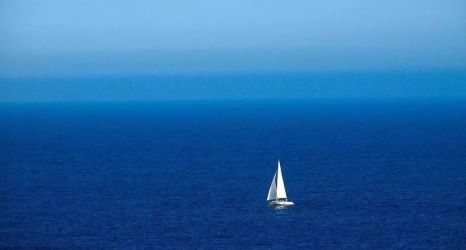
\includegraphics[width=3.5cm]{1.jpeg}
    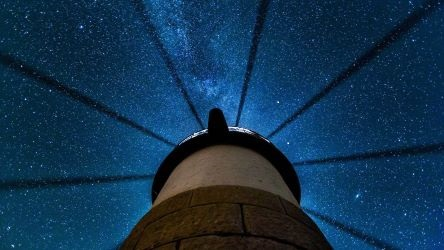
\includegraphics[width=3.5cm]{2.jpg}
    
\includegraphics[width=3.5cm]{3.jpg}
    \caption{实验数据集}
    \label{fig:data}
  \end{figure}
\end{frame}

\begin{frame}{实验结果分析}
  \begin{block}{评价指标}
    \begin{itemize}
      \item 相同迭代次数下的运行时间, 单位为秒.
      \item 低秩矩阵的秩 $\rank(\ml)$.
      \item 稀疏噪声矩阵的 0 范数 $\|\ms\|_0$.
      \item 目标函数值: 鲁棒主成分分析的目标函数值为
      \begin{equation}
        f=\|\ml\|_{*}+\lambda\|\ms\|_{m_1},\quad \lambda=\frac{1}{\sqrt{\max(m,n)}},
      \end{equation}
      矩阵补全的目标函数值为
      \begin{equation}
        f=\|\ml\|_{*}.
      \end{equation}
    \end{itemize}
  \end{block}
\end{frame}

\subsection{实验结果}

\subsubsection{主成分分析}

\begin{frame}{实验结果}
  \begin{block}{主成分分析}
    \begin{itemize}
      \item 主成分分析的实验结果如图 \ref{fig:results_pca}  所示.
      \item 第 1 行展示了原始图片与添加噪声后的图像, 其余行分别展示了 6 种不同超参数 (\textsf{r0}-\textsf{r5} 分别对应 $\rank(\ml)=[1,2,3,5,10,50]$) 下 PCA 算法的实验结果.
      \item 由图 \ref{fig:results_pca} 可知, 随着低秩矩阵秩的增加, 恢复出的低秩图像从仅有模糊背景到较清晰图像再到包含噪声图像逐渐转变, 而噪声图像中的元素逐渐减少趋于空白.
      \item 主成分分析算法的性能指标如表 \ref{tab:pca_index} 所示.
      \item 由表 \ref{tab:pca_index} 可知, 主成分分析算法所需的运行时间很短, 仅为 0.3 秒; 随着低秩矩阵秩的增加目标函数值先降低再增加.
    \end{itemize}
  \end{block}
\end{frame}

\begin{frame}{实验结果}
  \begin{figure}[H]
    \centering
    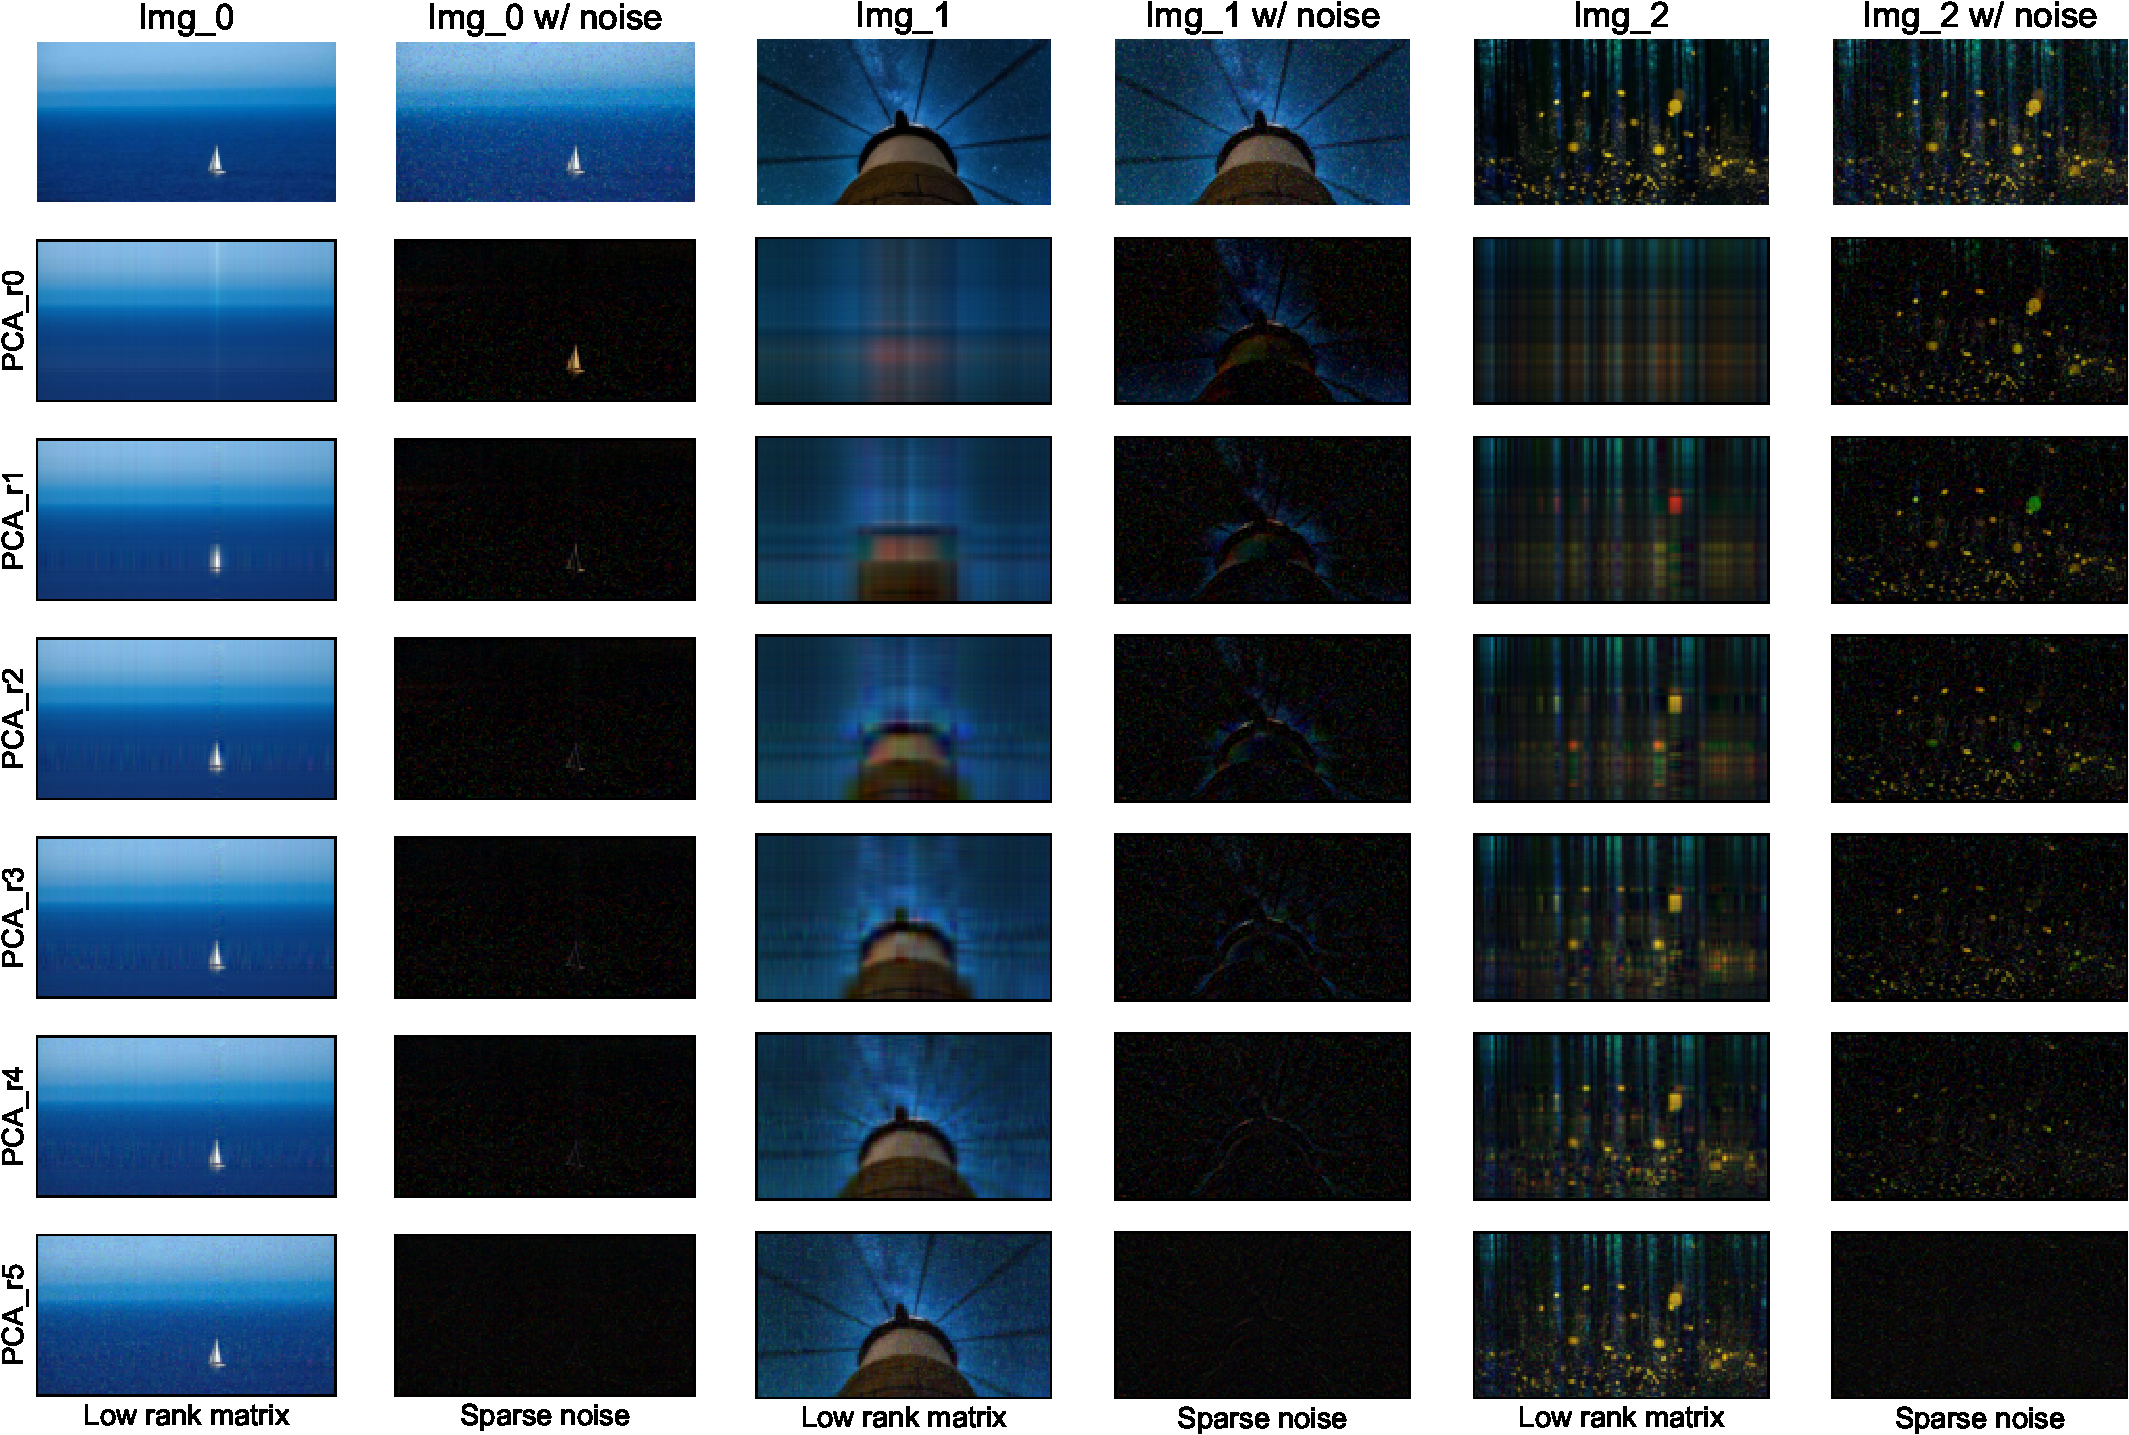
\includegraphics[height=6cm]{pca_total.pdf}
    \caption{主成分分析实验结果}
    \label{fig:results_pca}
  \end{figure}
\end{frame}

\begin{frame}{实验结果}
  \begin{table}[!htbp]
    \centering
    \small
    \caption{主成分分析算法性能指标}
    \label{tab:pca_index}
    \begin{tabular}{cccccc}
      \toprule
      Image & Algorithm     & Time (s)  & $\rank(\ml)$ & $\|\ms\|_0$  & $\|\ml\|_{*}+\lambda\|\ms\|_{m_1}$ \\
      \midrule
      0     & PCA r0    & 0.3      & 1.0         & 116500.0    & 398.6         \\
      0     & PCA r1    & 0.3      & 2.0         & 116500.0    & 398.1         \\
      0     & PCA r2    & 0.3      & 3.0         & 116500.0    & 408.5         \\
      0     & PCA r3    & 0.3      & 5.0         & 116500.0    & 428.2         \\
      0     & PCA r4    & 0.3      & 10.0        & 116500.0    & 476.6         \\
      0     & PCA r5    & 0.3      & 50.0        & 116500.0    & 679.1         \\
      1     & PCA r0    & 0.3      & 1.0         & 111000.0    & 570.8         \\
      1     & PCA r1    & 0.3      & 2.0         & 111000.0    & 486.9         \\
      1     & PCA r2    & 0.3      & 3.0         & 111000.0    & 478.5         \\
      \bottomrule
    \end{tabular}
  \end{table}
\end{frame}

\begin{frame}{实验结果}
  \centerline{(续表 \ref{tab:pca_index}: 主成分分析算法性能指标)}
  \begin{table}[H]
    \centering
    \small
    % \caption{主成分分析算法性能指标}
    % \label{tab:pca_index}
    \begin{tabular}{cccccc}
      \toprule
      Image & Algorithm     & Time (s)  & $\rank(\ml)$ & $\|\ms\|_0$  & $\|\ml\|_{*}+\lambda\|\ms\|_{m_1}$ \\
      \midrule
      1     & PCA r3    & 0.3      & 5.0         & 111000.0    & 475.1         \\
      1     & PCA r4    & 0.3      & 10.0        & 111000.0    & 498.5         \\
      1     & PCA r5    & 0.3      & 50.0        & 111000.0    & 679.6         \\
      2     & PCA r0    & 0.3      & 1.0         & 111000.0    & 514.5         \\
      2     & PCA r1    & 0.3      & 2.0         & 111000.0    & 501.9         \\
      2     & PCA r2    & 0.3      & 3.0         & 111000.0    & 496.9         \\
      2     & PCA r3    & 0.3      & 5.0         & 111000.0    & 502.6         \\
      2     & PCA r4    & 0.3      & 10.0        & 111000.0    & 528.8        \\
      2     & PCA r5    & 0.3      & 50.0        & 111000.0    & 717.7        \\
      \bottomrule
    \end{tabular}
  \end{table}
\end{frame}

\subsubsection{鲁棒主成分分析}

\begin{frame}{实验结果}
  \begin{block}{鲁棒主成分分析}
    \begin{itemize}
      \item 鲁棒主成分分析的实验结果如图 \ref{fig:results_rpca} 所示.
      \item 第 1 行展示了原始图片与添加噪声后的图像, 其余行分别展示了 Gradient descent (CGD), Gradient descent with Adam (CGD Adam), Augmented Lagrange multipliers (ALM), Singular value thresholding (SVT), Accelerated proximal gradient (APG) 算法的实验结果.
      \item 由图 \ref{fig:results_rpca} 可知, CGD, SVT 和 APG 算法的效果都比较好, ALM 算法在不同超参数下的效果差异比较明显.
    \end{itemize}
  \end{block}
\end{frame}

\begin{frame}{实验结果}
  \begin{figure}[!htbp]
    \centering
    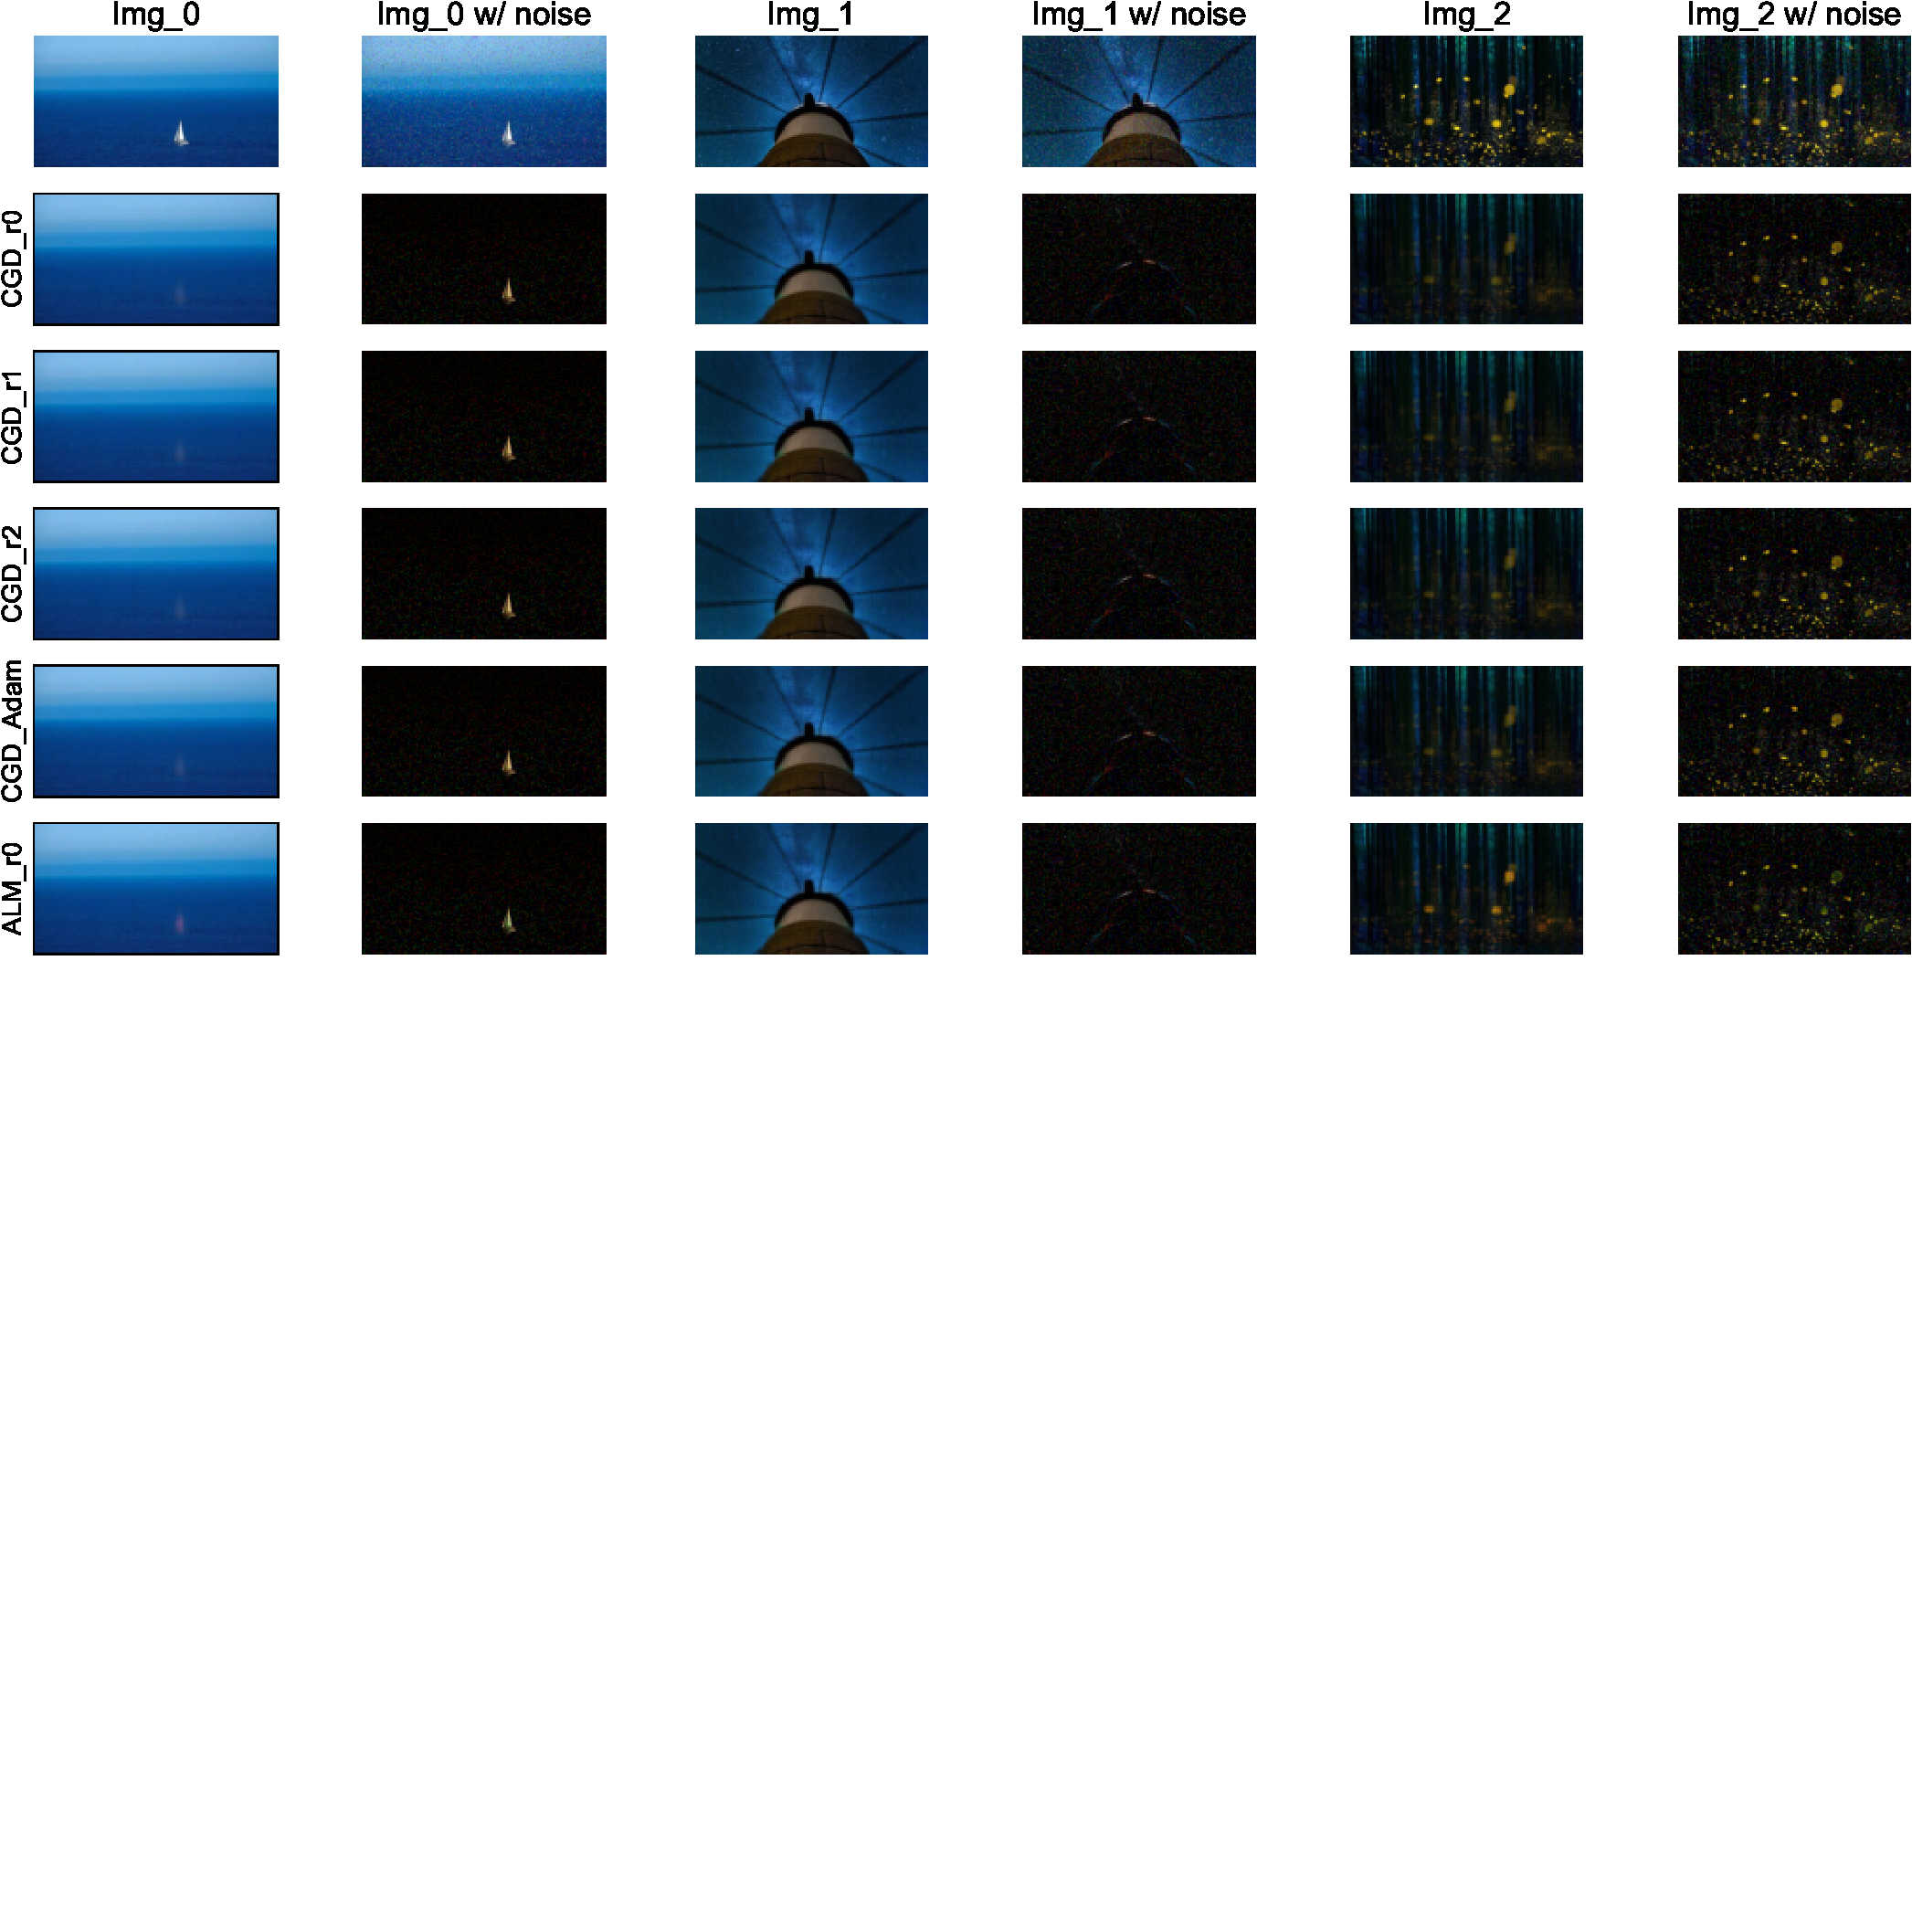
\includegraphics[height=5.5cm]{robust_pca_top.pdf}
    \caption{鲁棒主成分分析实验结果}
    \label{fig:results_rpca}
  \end{figure}
\end{frame}

\begin{frame}{实验结果}
  \begin{figure}[!htbp]
    \centering
    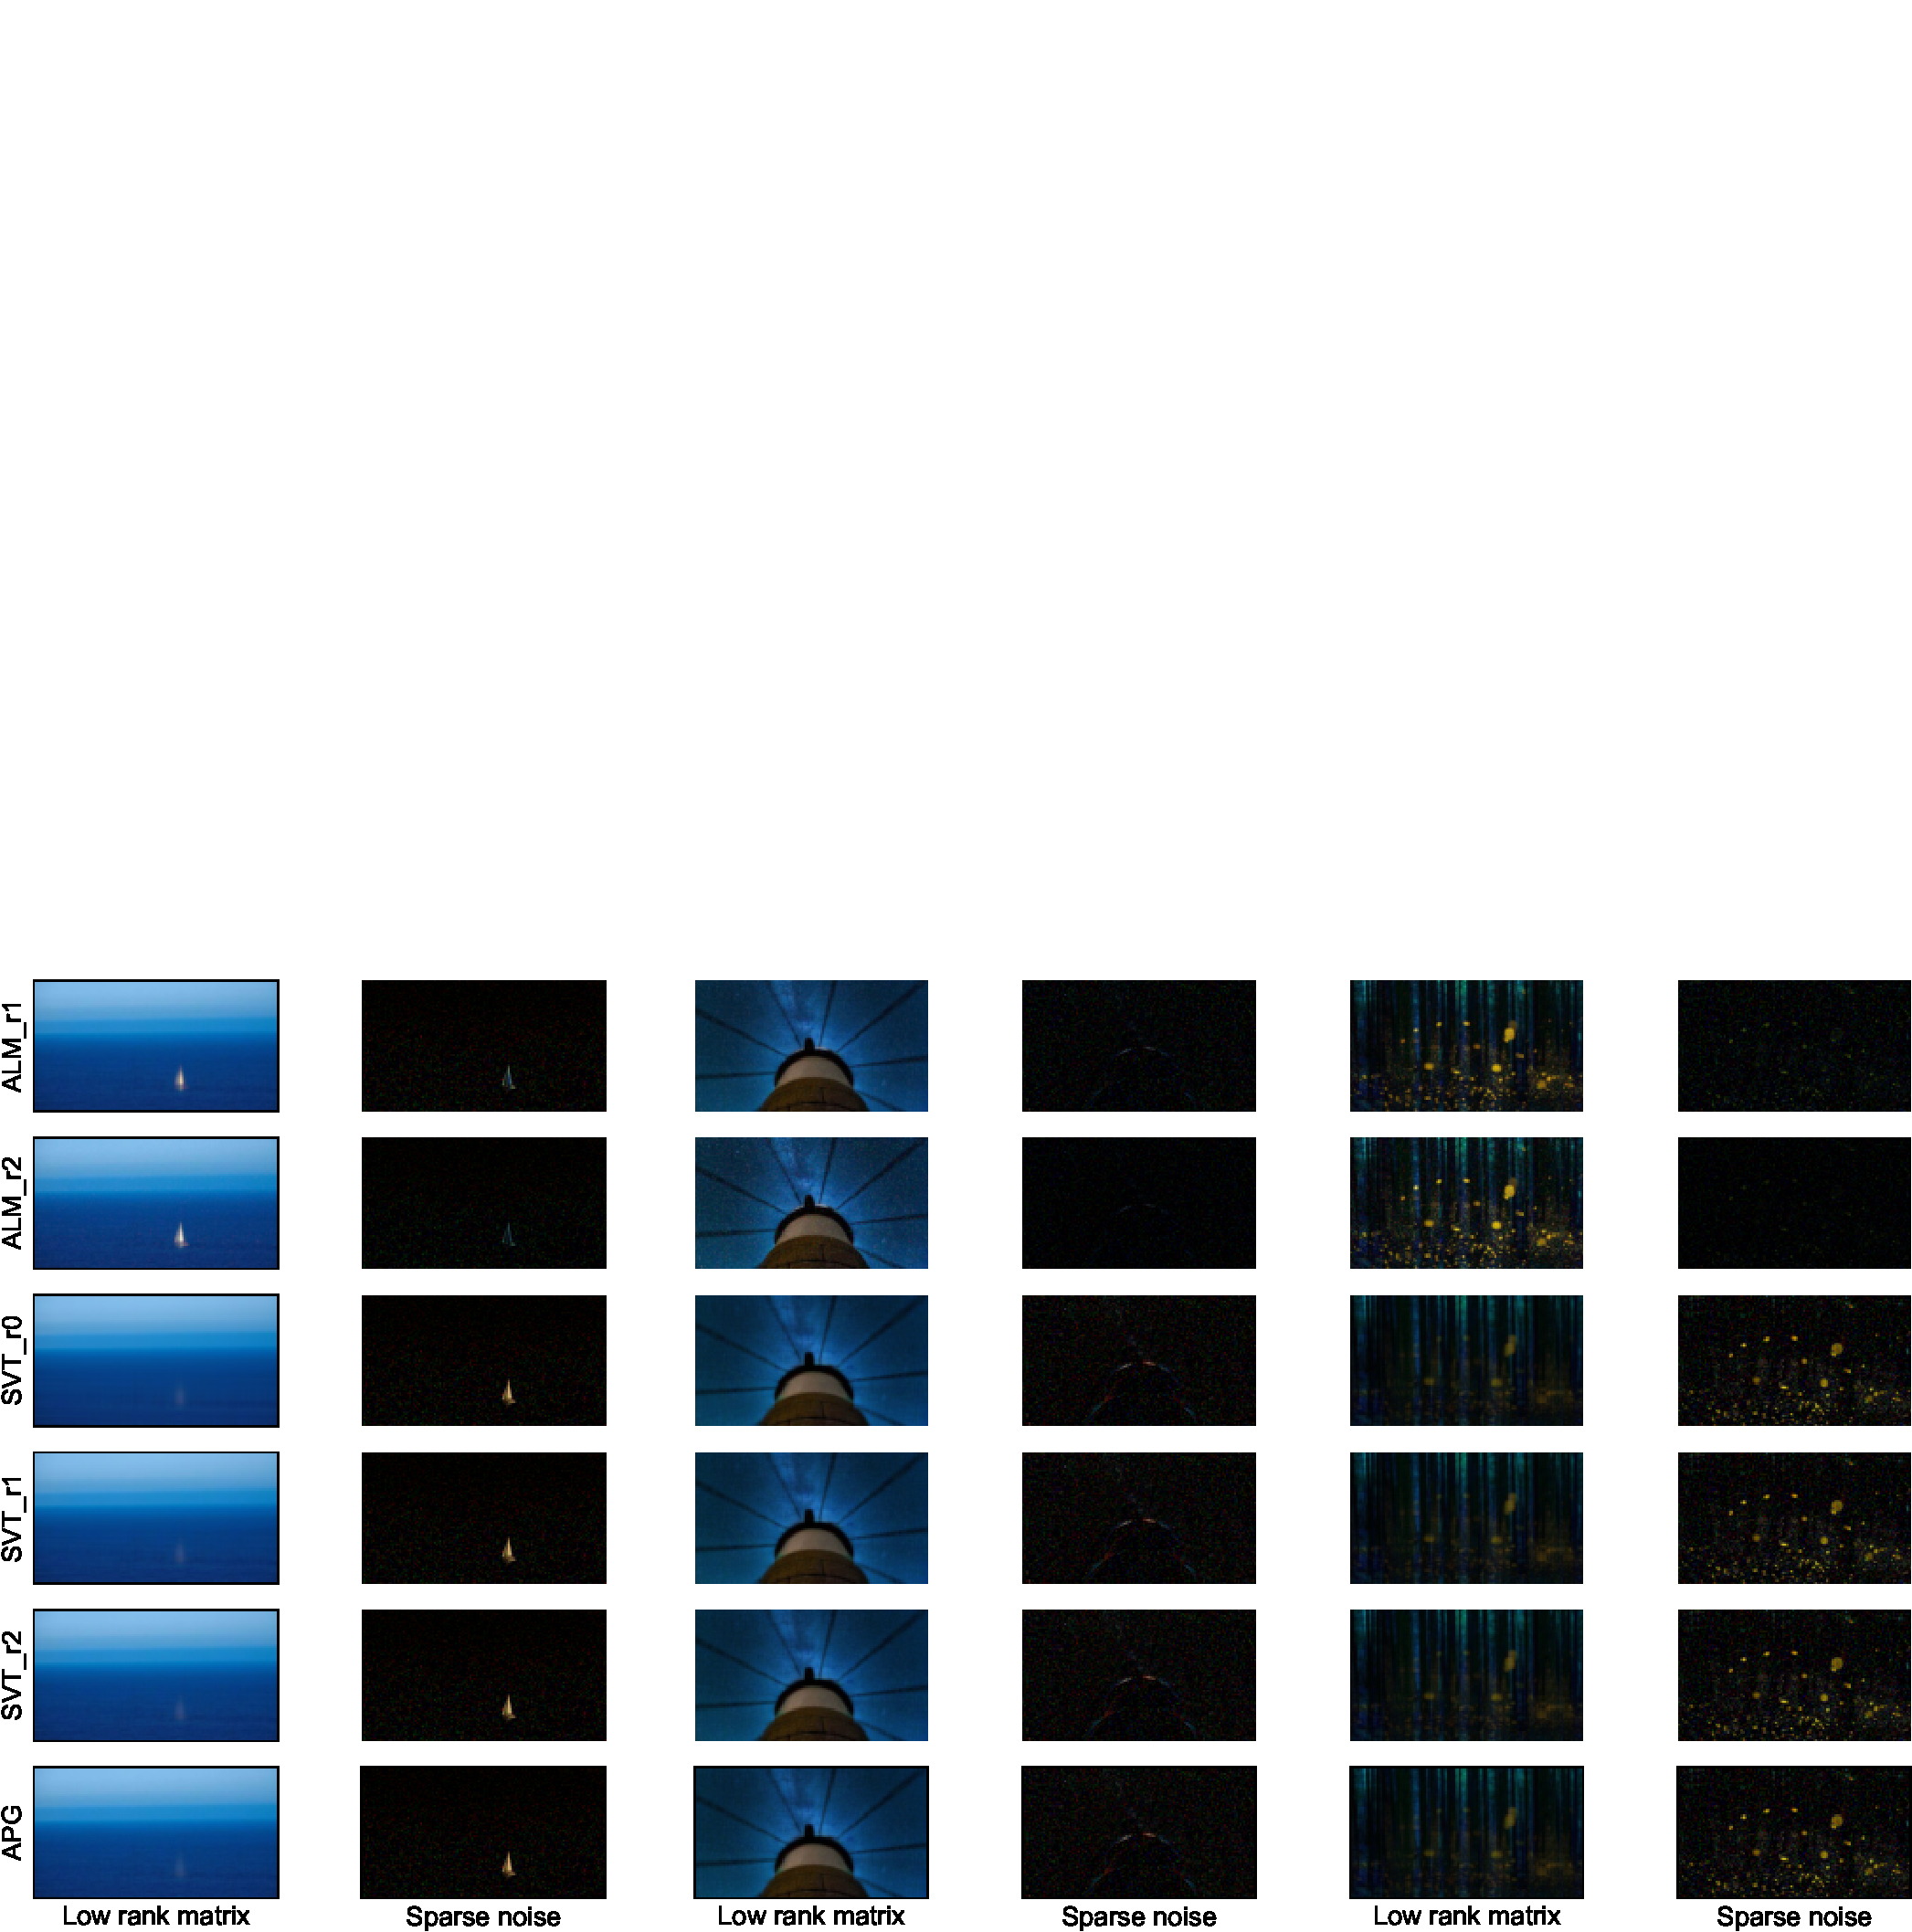
\includegraphics[height=5.5cm]{robust_pca_bottom.pdf}
    % \caption{鲁棒主成分分析实验结果}
    % \label{fig:results_rpca}
  \end{figure}
  \centerline{(续图 \ref{fig:results_rpca}: 鲁棒主成分分析实验结果)}
\end{frame}

\begin{frame}{实验结果}
  \begin{block}{超参数设置}
    图 \ref{fig:results_rpca} 左侧命名带有 \textsf{r0}, \textsf{r1}, \textsf{r2} 的算法为不同超参数的实验结果, 具体超参数设置如表 \ref{tab:rpca_hyperparams} 所示.
  \end{block}
  \begin{table}[H]
    \centering
    \small
    \caption{鲁棒主成分分析各算法超参数设置}
    \label{tab:rpca_hyperparams}
    \begin{tabular}{cccc}
      \toprule
      Algorithm  & \textsf{r0}  & \textsf{r1} & \textsf{r2}  \\
      \midrule
      CGD & $\mu\leftarrow0.0005\mu$ & $\mu\leftarrow0.001\mu$ & $\mu\leftarrow0.005\mu$ \\
      ALM & $\mu\leftarrow0.1\mu$ & $\mu\leftarrow0.5\mu$ & $\mu\leftarrow\mu$ \\
      SVT & $\mu=\alpha=0.001$ & $\mu=\alpha=0.002$ & $\mu=\alpha=0.003$ \\
      \bottomrule
    \end{tabular}
  \end{table}
\end{frame}

\begin{frame}{实验结果}
  \begin{block}{性能指标}
    \begin{itemize}
      \item 鲁棒主成分分析算法的性能指标如表 \ref{tab:rpca_index} 所示. 
      \item 由表 \ref{tab:rpca_index} 可知, CGD 算法的运行时间显著高于其他 3 个算法, 而且几乎没有达到降秩的结果.
      \item 但是 CGD 算法得到的低秩图像和稀疏噪声图像的视觉效果还不错, 所以绝对意义上的降秩并不是达到预期效果的必要条件.
      \item SVT 算法的降秩效果最好, 而且噪声矩阵的稀疏性也最好, 因此其目标函数值也是最小的.
    \end{itemize}
  \end{block}
\end{frame}

\begin{frame}{实验结果}
  \begin{table}[H]
    \vspace*{-5.27pt}
    \centering
    \scriptsize
    \caption{鲁棒主成分分析各算法性能指标}
    \label{tab:rpca_index}
    \begin{tabular}{cccccc}
      \toprule
      Image & Algorithm      & Time (s)  & $\rank(\ml)$ & $\|\ms\|_0$    & $\|\ml\|_{*}+\lambda\|\ms\|_{m_1}$ \\
      \midrule
      0     & ALM r0    & 330.7    & 136.3       & 73402.3     & 333.2         \\
      0     & ALM r1    & 329.4    & 141.0       & 72262.0     & 335.3         \\
      0     & ALM r2    & 327.6    & 184.0       & 51798.0     & 385.6         \\
      0     & APG       & 328.0    & 135.7       & 73546.7     & 333.1         \\
      0     & SVT r0    & 322.8    & 4.0         & 6249.3      & 303.3         \\
      0     & SVT r1    & 327.1    & 14.7        & 10840.3     & 313.5         \\
      0     & SVT r2    & 325.6    & 27.7        & 16095.7     & 320.0         \\
      0     & CGD r0    & 535.9    & 250.0       & 116500.0    & 333.2         \\
      0     & CGD r1    & 534.2    & 250.0       & 116500.0    & 333.3         \\
      0     & CGD r2    & 537.1    & 250.0       & 116500.0    & 333.5         \\
      0     & CGD Adam  & 532.9    & 250.0       & 116500.0    & 347.9         \\
      1     & ALM r0    & 260.1    & 140.0       & 72664.0     & 388.1         \\
      1     & ALM r1    & 263.1    & 207.0       & 51589.3     & 425.6         \\
      1     & ALM r2    & 266.7    & 248.0       & 26648.7     & 533.6         \\
      1     & APG       & 262.4    & 141.7       & 73975.7     & 388.1         \\
      1     & SVT r0    & 261.9    & 28.3        & 20876.3     & 335.5         \\
      1     & SVT r1    & 263.6    & 63.7        & 38295.0     & 367.9         \\
      \bottomrule
    \end{tabular}
  \end{table}
\end{frame}

\begin{frame}{实验结果}
  \centerline{(续表 \ref{tab:rpca_index} : 鲁棒主成分分析各算法性能指标)}
  \begin{table}[H]
    \centering
    \scriptsize
    % \caption{鲁棒主成分分析各算法性能指标}
    % \label{tab:rpca_index}
    \begin{tabular}{cccccc}
      \toprule
      Image & Algorithm      & Time (s)  & $\rank(\ml)$ & $\|\ms\|_0$    & $\|\ml\|_{*}+\lambda\|\ms\|_{m_1}$ \\
      \midrule
      1     & SVT r1    & 263.6    & 63.7        & 38295.0     & 367.9         \\
      1     & SVT r2    & 265.8    & 85.7        & 48169.7     & 378.1         \\
      1     & CGD r0    & 463.2    & 250.0       & 111000.0    & 388.2         \\
      1     & CGD r1    & 464.9    & 250.0       & 111000.0    & 388.4         \\
      1     & CGD r2    & 466.6    & 250.0       & 111000.0    & 388.6         \\
      1     & CGD Adam  & 468.0    & 250.0       & 111000.0    & 404.4         \\
      2     & ALM r0    & 261.9    & 141.7       & 72063.3     & 374.4         \\
      2     & ALM r1    & 261.2    & 232.3       & 40029.3     & 462.0         \\
      2     & ALM r2    & 268.4    & 250.0       & 19075.7     & 608.6         \\
      2     & APG       & 266.9    & 141.7       & 74387.0     & 373.5         \\
      2     & SVT r0    & 265.1    & 33.7        & 23243.7     & 331.7         \\
      2     & SVT r1    & 263.1    & 58.7        & 36326.7     & 355.5         \\
      2     & SVT r2    & 262.7    & 76.0        & 43697.3     & 363.4         \\
      2     & CGD r0    & 463.7    & 250.0       & 111000.0    & 373.7         \\
      2     & CGD r1    & 465.7    & 250.0       & 111000.0    & 373.9         \\
      2     & CGD r2    & 466.2    & 250.0       & 111000.0    & 374.1         \\
      2     & CGD Adam  & 470.6    & 250.0       & 111000.0    & 395.3        \\
      \bottomrule
    \end{tabular}
  \end{table}
\end{frame}

\subsubsection{矩阵补全}

\begin{frame}{实验结果}
  \begin{block}{矩阵补全}
    \begin{itemize}
      \item 矩阵补全的实验结果如图 \ref{fig:results_mc} 所示, 其中第 1 行展示了原始图片与添加噪声后的图像, 其余行分别展示了 Alternating direction method (ADMM), Singular value thresholding (SVT), Alternating least squares (PMF, BPMF) 算法的实验结果.
      \item 由图 \ref{fig:results_mc} 可知, ADMM 和 SVT 算法的效果都比较好, PMF 和 BPMF 算法的效果则要差一些.
      \item 矩阵补全 CNTK 方法的实验结果如图 \ref{fig:results_mc_ntk} 所示, 其中第 1 行展示了原始图片与添加噪声后的图像, 第 2 行是直接使用 CNTK 方法得到的结果, 第 3 行展示使用 CNTK 和 EigenPro 得到的结果. 
      \item 由图 \ref{fig:results_mc_ntk} 可知, CNTK 方法得到的结果都比较不错.
    \end{itemize}
  \end{block}
\end{frame}

\begin{frame}{实验结果}
  \begin{figure}[H]
    \centering
    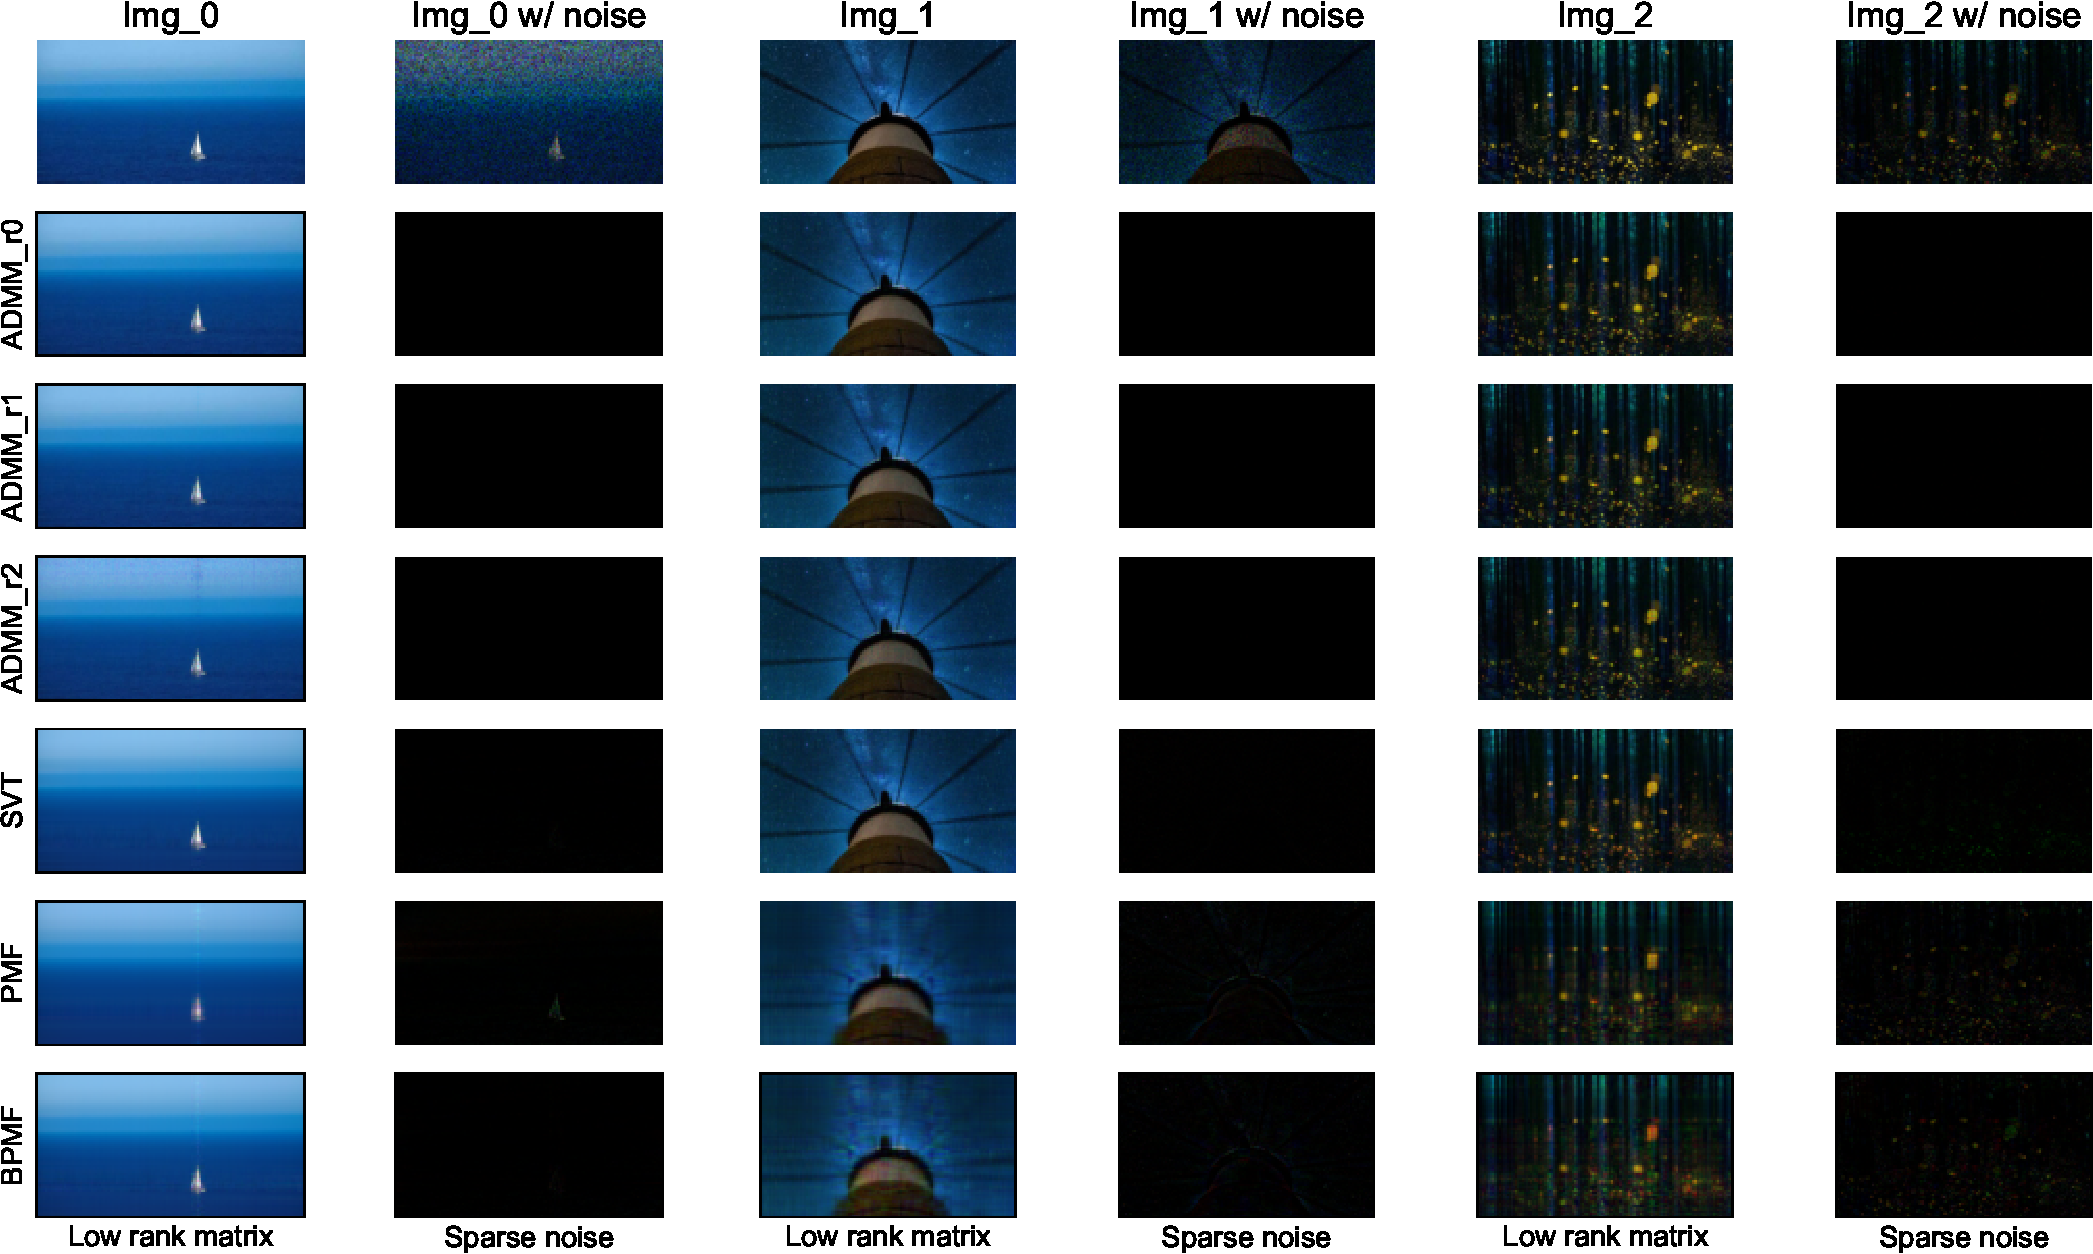
\includegraphics[height=6cm]{matrix_completion.pdf}
    \caption{矩阵补全实验结果}
    \label{fig:results_mc}
  \end{figure}
\end{frame}

\begin{frame}{实验结果}
  \begin{figure}[H]
    \centering
    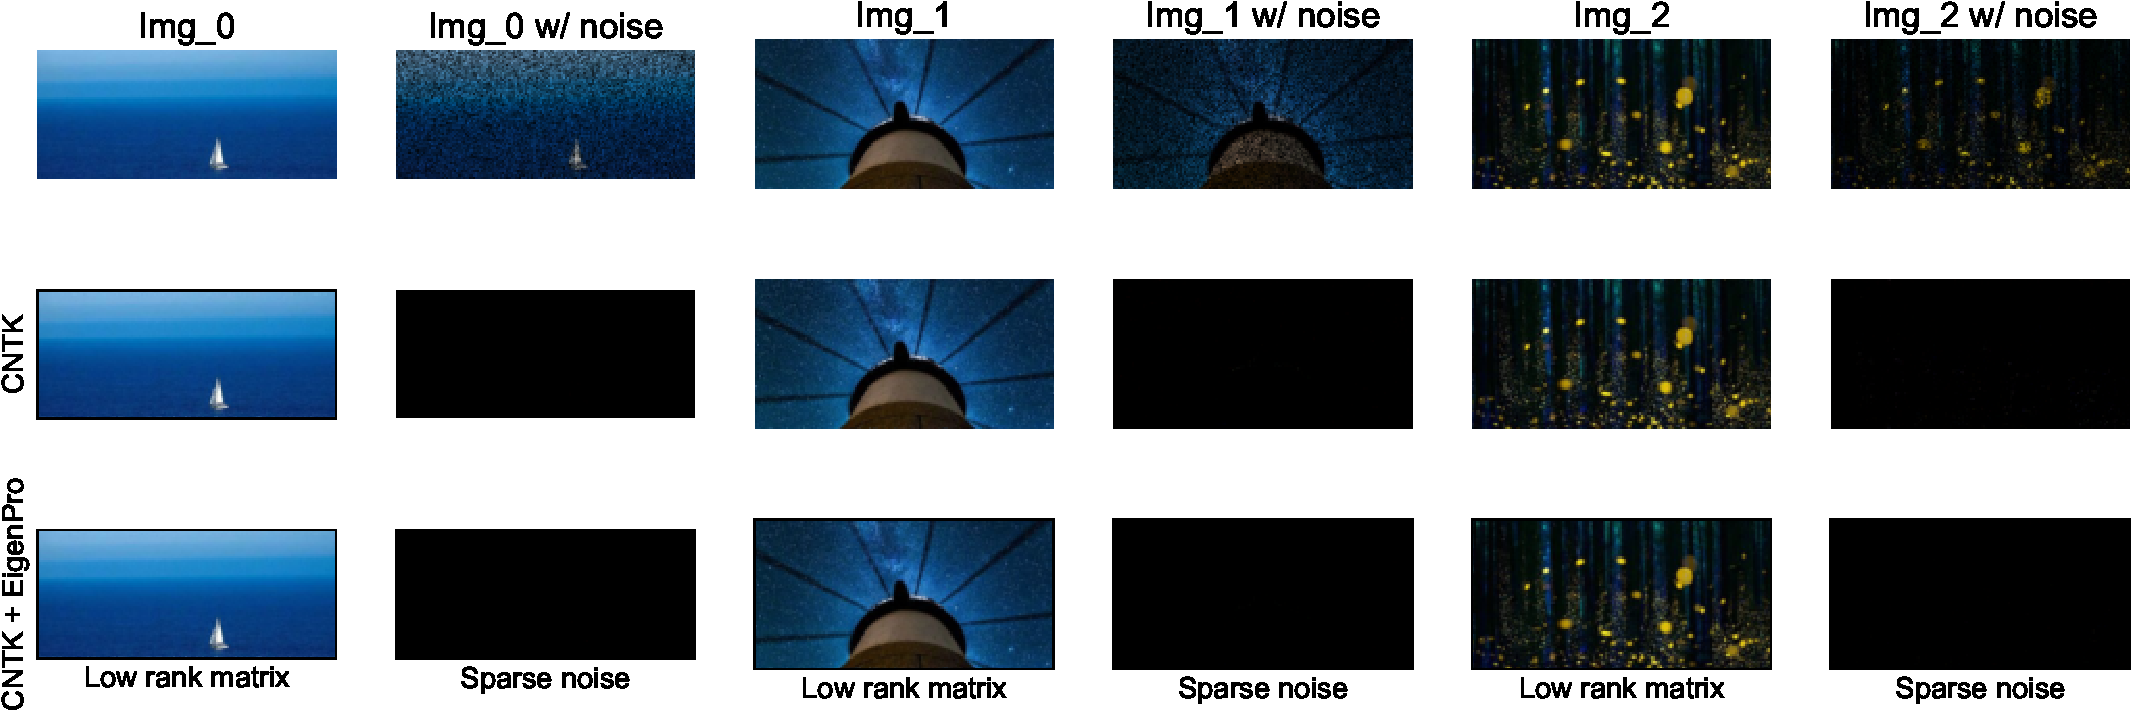
\includegraphics[height=3.6cm]{matrix_completion_ntk.pdf}
    \caption{矩阵补全 CNTK 方法实验结果}
    \label{fig:results_mc_ntk}
  \end{figure}
\end{frame}

\begin{frame}{实验结果}
  \begin{block}{超参数设置}
    图 \ref{fig:results_mc} 左侧命名带有 \textsf{r0}, \textsf{r1}, \textsf{r2} 的算法为不同超参数的实验结果, 具体超参数设置如表 \ref{tab:mc_hyperparams} 所示.
  \end{block}
  \begin{table}[H]
    \centering
    \small
    \caption{矩阵补全算法超参数设置}
    \label{tab:mc_hyperparams}
    \begin{tabular}{cccc}
      \toprule
      Algorithm  & \textsf{r0}  & \textsf{r1} & \textsf{r2}  \\
      \midrule
      ADMM & $\mu\leftarrow0.05\mu$ & $\mu\leftarrow0.1\mu$ & $\mu\leftarrow0.15\mu$ \\
      \bottomrule
    \end{tabular}
  \end{table}
\end{frame}

\begin{frame}{实验结果}
  \begin{block}{性能指标}
    \begin{itemize}
      \item 矩阵补全算法的性能指标如表 \ref{tab:mc_index} 所示.
      \item 由表 \ref{tab:mc_index} 可知, ADMM 和 CNTK 算法的运行时间显著多于其他算法, 使用了 EigenPro 的 CNTK 算法的运行时间显著减少.
      \item SVT, PMF 和 BPMF 算法得到的低秩矩阵的秩均比较小, 但是噪声矩阵的稀疏性较差.
    \end{itemize}
  \end{block}
\end{frame}

\begin{frame}{实验结果}
  \begin{table}[H]
    \centering
    \small
    \caption{矩阵补全各算法性能指标}
    \label{tab:mc_index}
    \begin{tabular}{cccccc}
      \toprule
      Image & Algorithm     & Time (s)  & $\rank(\ml)$ & $\|\ms\|_0$  & $\|\ml\|_{*}$ \\
      \midrule
      0     & ADMM r0       & 322.6    & 191.7       & 57822.7     & 206.2         \\
      0     & ADMM r1       & 330.4    & 192.0       & 57822.7     & 206.4         \\
      0     & ADMM r2       & 325.9    & 198.0       & 57822.7     & 239.7         \\
      0     & SVT           & 36.3     & 8.7         & 116500.0    & 178.0         \\
      0     & PMF           & 2.0      & 10.0        & 116500.0    & 164.1         \\
      0     & BPMF          & 2.0      & 12.0        & 116500.0    & 180.7         \\
      0     & CNTK          & 340.7    & 192.0       & 43120.0     & 181.4         \\
      0     & CNTK EigenPro & 69.1     & 192.0       & 43120.0     & 180.0         \\
      1     & ADMM r0       & 263.3    & 196.7       & 53239.3     & 262.9         \\
      1     & ADMM r1       & 266.2    & 200.0       & 53239.3     & 263.7         \\
      1     & ADMM r2       & 261.0    & 205.0       & 53239.3     & 269.6         \\
      1     & SVT           & 297.5    & 58.7        & 111000.0    & 208.4         \\
      \bottomrule
    \end{tabular}
  \end{table}
\end{frame}

\begin{frame}{实验结果}
  \centerline{(续表 \ref{tab:mc_index}: 矩阵补全各算法性能指标)}
  \begin{table}[H]
    \centering
    \small
    % \caption{矩阵补全各算法性能指标}
    % \label{tab:mc_index}
    \begin{tabular}{cccccc}
      \toprule
      Image & Algorithm     & Time (s)  & $\rank(\ml)$ & $\|\ms\|_0$  & $\|\ml\|_{*}$ \\
      \midrule
      1     & PMF           & 1.8      & 10.0        & 111000.0    & 120.6         \\
      1     & BPMF          & 1.9      & 12.0        & 111000.0    & 131.3         \\
      1     & CNTK          & 340.7    & 192.0       & 36756.0     & 238.2         \\
      1     & CNTK EigenPro & 69.1     & 192.0       & 36755.7     & 225.8         \\
      2     & ADMM r0       & 261.5    & 200.7       & 50828.0     & 282.4         \\
      2     & ADMM r1       & 263.2    & 204.0       & 50828.0     & 283.7         \\
      2     & ADMM r2       & 262.5    & 208.0       & 50828.0     & 286.6         \\
      2     & SVT           & 730.6    & 83.3        & 111000.0    & 210.7         \\
      2     & PMF           & 1.9      & 10.0        & 111000.0    & 80.4          \\
      2     & BPMF          & 1.9      & 12.0        & 111000.0    & 95.2          \\
      2     & CNTK          & 340.7    & 192.0       & 36746.0     & 253.3         \\
      2     & CNTK EigenPro & 69.1     & 192.0       & 36746.0     & 236.3        \\
      \bottomrule
    \end{tabular}
  \end{table}
\end{frame}

\section[代码]{代码说明}

\begin{frame}{代码说明}
  \begin{block}{参考代码}
    \begin{itemize}
      \item 本文参考的代码如表 \ref{tab:code_refs} 所示, 这些代码文件的位置为: \texttt{utils/}.
      \item \texttt{ntk/} 文件夹为文献 \cite{radhakrishnan2022simple} 作者提供的 CNTK 方法的开源代码, 本文基于该开源代码进行了简单修改, 以用于本任务.
    \end{itemize}
  \end{block}
  \begin{table}[H]
    \centering
    \tiny
    \caption{参考代码及链接}
    \label{tab:code_refs}
    \begin{tabular}{lll}
      \toprule
      file & function       & link   \\
      \midrule
      \texttt{robust\_pca.py}    & \texttt{\_augmented\_Lagrange\_multipliers()} & \href{https://github.com/dganguli/robust-pca}{\color{purple}Robust-PCA}   \\
      \texttt{matrix\_completion.py}    & \texttt{\_singular\_value\_thresholding()} & \href{https://github.com/tonyduan/matrix-completion}{\color{purple}matrix-completion}   \\
      \texttt{matrix\_completion.py}    & \texttt{\_probabilistic\_matrix\_factorization()} & \href{https://github.com/tonyduan/matrix-completion}{\color{purple}matrix-completion}   \\
      \texttt{matrix\_completion.py}    & \texttt{\_biased\_probabilistic\_matrix\_factorization()} & \href{https://github.com/tonyduan/matrix-completion}{\color{purple}matrix-completion}   \\
      \bottomrule
    \end{tabular}
  \end{table}
\end{frame}

\begin{frame}{代码说明}
  \begin{block}{代码结构}
    代码结构如表 \ref{tab:code_framework} 所示, 其中核心算法位于 \texttt{utils/} 文件夹.
  \end{block}
  \begin{table}[H]
    \centering
    \scriptsize
    \caption{代码结构}
    \label{tab:code_framework}
    \begin{tabular}{lll}
      \toprule
      folder & description    \\
      \midrule
      \texttt{bin/}    &  testing algorithms, analyzing results, and plotting figures   \\
      \texttt{data/}    &  source data and results   \\
      \texttt{doc/}    &  documentation   \\
      \texttt{ntk/}    &  the CNTK algorithm   \\
      \texttt{pre/}    &  slides   \\
      \texttt{utils/}    &  algorithms   \\
      \bottomrule
    \end{tabular}
  \end{table}
\end{frame}

\section[贡献]{贡献说明}

\begin{frame}{贡献说明}
  本研究的分工如表 \ref{tab:contribution} 所示.

  \begin{table}[htbp]
    \centering
    \small
    \caption{贡献说明}
    \label{tab:contribution}
    \begin{tabular}{lll}
      \toprule
      工作内容 & 完成人    \\
      \midrule
      鲁棒主成分分析: 通用算法 & 杨敬轩 \\
      鲁棒主成分分析: 特殊算法 & 杨敬轩 \\
      矩阵补全算法 & 董泽委 \\
      实验结果分析 & 杨敬轩, 董泽委 (1: 0.9) \\
      报告撰写 & 杨敬轩, 董泽委 (1: 0.7) \\
      Beamer 制作 & 杨敬轩, 董泽委 (1: 0.5) \\
      \bottomrule
    \end{tabular}
  \end{table}
\end{frame}

\section{参考文献}

\begin{frame}[allowframebreaks]{参考文献}
  \footnotesize
  \bibliography{ref}
  \bibliographystyle{unsrt}
\end{frame}

\begin{frame}
  \begin{center}
    {\Huge\calligra Thanks for your attention!}
    \vspace{1cm}

    {\Huge Q \& A}
  \end{center}
\end{frame}

\end{document}
